% Created by tikzDevice version 0.12 on 2018-10-15 14:29:31
% !TEX encoding = UTF-8 Unicode
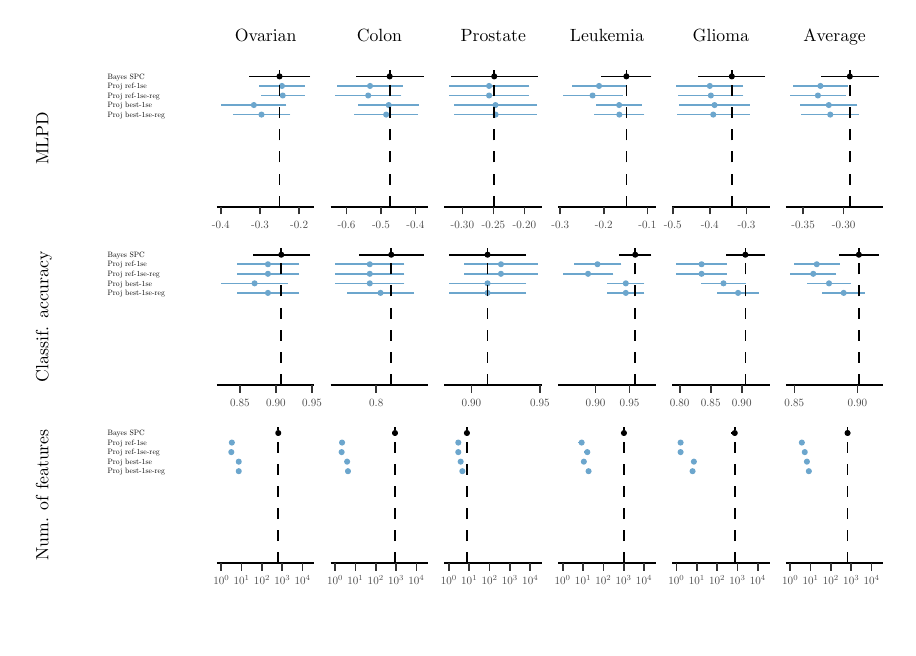
\begin{tikzpicture}[x=1pt,y=1pt]
\definecolor{fillColor}{RGB}{255,255,255}
\path[use as bounding box,fill=fillColor,fill opacity=0.00] (0,0) rectangle (310.76,216.81);
\begin{scope}
\path[clip] (  0.00,204.19) rectangle (  9.80,216.81);
\definecolor{drawColor}{RGB}{255,255,255}
\definecolor{fillColor}{RGB}{255,255,255}

\path[draw=drawColor,line width= 0.6pt,line join=round,line cap=round,fill=fillColor] (  0.00,204.19) rectangle (  9.80,216.81);
\end{scope}
\begin{scope}
\path[clip] (  0.00,139.76) rectangle (  9.80,204.19);
\definecolor{drawColor}{RGB}{255,255,255}
\definecolor{fillColor}{RGB}{255,255,255}

\path[draw=drawColor,line width= 0.6pt,line join=round,line cap=round,fill=fillColor] (  0.00,139.76) rectangle (  9.80,204.19);
\end{scope}
\begin{scope}
\path[clip] (  0.00, 75.32) rectangle (  9.80,139.76);
\definecolor{drawColor}{RGB}{255,255,255}
\definecolor{fillColor}{RGB}{255,255,255}

\path[draw=drawColor,line width= 0.6pt,line join=round,line cap=round,fill=fillColor] (  0.00, 75.32) rectangle (  9.80,139.76);
\end{scope}
\begin{scope}
\path[clip] (  0.00,  0.00) rectangle (  9.80, 75.32);
\definecolor{drawColor}{RGB}{255,255,255}
\definecolor{fillColor}{RGB}{255,255,255}

\path[draw=drawColor,line width= 0.6pt,line join=round,line cap=round,fill=fillColor] (  0.00,  0.00) rectangle (  9.80, 75.32);
\end{scope}
\begin{scope}
\path[clip] (  9.80,204.19) rectangle ( 64.06,216.81);
\definecolor{drawColor}{RGB}{255,255,255}
\definecolor{fillColor}{RGB}{255,255,255}

\path[draw=drawColor,line width= 0.6pt,line join=round,line cap=round,fill=fillColor] (  9.80,204.19) rectangle ( 64.06,216.81);
\end{scope}
\begin{scope}
\path[clip] (  9.80,139.76) rectangle ( 64.06,204.19);
\definecolor{drawColor}{RGB}{255,255,255}
\definecolor{fillColor}{RGB}{255,255,255}

\path[draw=drawColor,line width= 0.6pt,line join=round,line cap=round,fill=fillColor] (  9.80,139.76) rectangle ( 64.06,204.19);
\end{scope}
\begin{scope}
\path[clip] (  9.80, 75.32) rectangle ( 64.06,139.76);
\definecolor{drawColor}{RGB}{255,255,255}
\definecolor{fillColor}{RGB}{255,255,255}

\path[draw=drawColor,line width= 0.6pt,line join=round,line cap=round,fill=fillColor] (  9.80, 75.32) rectangle ( 64.06,139.76);
\end{scope}
\begin{scope}
\path[clip] (  9.80,  0.00) rectangle ( 64.06, 75.32);
\definecolor{drawColor}{RGB}{255,255,255}
\definecolor{fillColor}{RGB}{255,255,255}

\path[draw=drawColor,line width= 0.6pt,line join=round,line cap=round,fill=fillColor] (  9.80,  0.00) rectangle ( 64.06, 75.32);
\end{scope}
\begin{scope}
\path[clip] ( 64.06,204.19) rectangle (105.18,216.81);
\definecolor{drawColor}{RGB}{255,255,255}
\definecolor{fillColor}{RGB}{255,255,255}

\path[draw=drawColor,line width= 0.6pt,line join=round,line cap=round,fill=fillColor] ( 64.06,204.19) rectangle (105.18,216.81);
\end{scope}
\begin{scope}
\path[clip] ( 64.06,139.76) rectangle (105.18,204.19);
\definecolor{drawColor}{RGB}{255,255,255}
\definecolor{fillColor}{RGB}{255,255,255}

\path[draw=drawColor,line width= 0.6pt,line join=round,line cap=round,fill=fillColor] ( 64.06,139.76) rectangle (105.18,204.19);
\end{scope}
\begin{scope}
\path[clip] ( 64.06, 75.32) rectangle (105.18,139.76);
\definecolor{drawColor}{RGB}{255,255,255}
\definecolor{fillColor}{RGB}{255,255,255}

\path[draw=drawColor,line width= 0.6pt,line join=round,line cap=round,fill=fillColor] ( 64.06, 75.32) rectangle (105.18,139.76);
\end{scope}
\begin{scope}
\path[clip] ( 64.06,  0.00) rectangle (105.18, 75.32);
\definecolor{drawColor}{RGB}{255,255,255}
\definecolor{fillColor}{RGB}{255,255,255}

\path[draw=drawColor,line width= 0.6pt,line join=round,line cap=round,fill=fillColor] ( 64.06,  0.00) rectangle (105.18, 75.32);
\end{scope}
\begin{scope}
\path[clip] (105.18,204.19) rectangle (146.29,216.81);
\definecolor{drawColor}{RGB}{255,255,255}
\definecolor{fillColor}{RGB}{255,255,255}

\path[draw=drawColor,line width= 0.6pt,line join=round,line cap=round,fill=fillColor] (105.18,204.19) rectangle (146.29,216.81);
\end{scope}
\begin{scope}
\path[clip] (105.18,139.76) rectangle (146.29,204.19);
\definecolor{drawColor}{RGB}{255,255,255}
\definecolor{fillColor}{RGB}{255,255,255}

\path[draw=drawColor,line width= 0.6pt,line join=round,line cap=round,fill=fillColor] (105.18,139.76) rectangle (146.29,204.19);
\end{scope}
\begin{scope}
\path[clip] (105.18, 75.32) rectangle (146.29,139.76);
\definecolor{drawColor}{RGB}{255,255,255}
\definecolor{fillColor}{RGB}{255,255,255}

\path[draw=drawColor,line width= 0.6pt,line join=round,line cap=round,fill=fillColor] (105.18, 75.32) rectangle (146.29,139.76);
\end{scope}
\begin{scope}
\path[clip] (105.18,  0.00) rectangle (146.29, 75.32);
\definecolor{drawColor}{RGB}{255,255,255}
\definecolor{fillColor}{RGB}{255,255,255}

\path[draw=drawColor,line width= 0.6pt,line join=round,line cap=round,fill=fillColor] (105.18,  0.00) rectangle (146.29, 75.32);
\end{scope}
\begin{scope}
\path[clip] (146.29,204.19) rectangle (187.41,216.81);
\definecolor{drawColor}{RGB}{255,255,255}
\definecolor{fillColor}{RGB}{255,255,255}

\path[draw=drawColor,line width= 0.6pt,line join=round,line cap=round,fill=fillColor] (146.29,204.19) rectangle (187.41,216.81);
\end{scope}
\begin{scope}
\path[clip] (146.29,139.76) rectangle (187.41,204.19);
\definecolor{drawColor}{RGB}{255,255,255}
\definecolor{fillColor}{RGB}{255,255,255}

\path[draw=drawColor,line width= 0.6pt,line join=round,line cap=round,fill=fillColor] (146.29,139.76) rectangle (187.41,204.19);
\end{scope}
\begin{scope}
\path[clip] (146.29, 75.32) rectangle (187.41,139.76);
\definecolor{drawColor}{RGB}{255,255,255}
\definecolor{fillColor}{RGB}{255,255,255}

\path[draw=drawColor,line width= 0.6pt,line join=round,line cap=round,fill=fillColor] (146.29, 75.32) rectangle (187.41,139.76);
\end{scope}
\begin{scope}
\path[clip] (146.29,  0.00) rectangle (187.41, 75.32);
\definecolor{drawColor}{RGB}{255,255,255}
\definecolor{fillColor}{RGB}{255,255,255}

\path[draw=drawColor,line width= 0.6pt,line join=round,line cap=round,fill=fillColor] (146.29,  0.00) rectangle (187.41, 75.32);
\end{scope}
\begin{scope}
\path[clip] (187.41,204.19) rectangle (228.53,216.81);
\definecolor{drawColor}{RGB}{255,255,255}
\definecolor{fillColor}{RGB}{255,255,255}

\path[draw=drawColor,line width= 0.6pt,line join=round,line cap=round,fill=fillColor] (187.41,204.19) rectangle (228.53,216.81);
\end{scope}
\begin{scope}
\path[clip] (187.41,139.76) rectangle (228.53,204.19);
\definecolor{drawColor}{RGB}{255,255,255}
\definecolor{fillColor}{RGB}{255,255,255}

\path[draw=drawColor,line width= 0.6pt,line join=round,line cap=round,fill=fillColor] (187.41,139.76) rectangle (228.53,204.19);
\end{scope}
\begin{scope}
\path[clip] (187.41, 75.32) rectangle (228.53,139.76);
\definecolor{drawColor}{RGB}{255,255,255}
\definecolor{fillColor}{RGB}{255,255,255}

\path[draw=drawColor,line width= 0.6pt,line join=round,line cap=round,fill=fillColor] (187.41, 75.32) rectangle (228.53,139.76);
\end{scope}
\begin{scope}
\path[clip] (187.41,  0.00) rectangle (228.53, 75.32);
\definecolor{drawColor}{RGB}{255,255,255}
\definecolor{fillColor}{RGB}{255,255,255}

\path[draw=drawColor,line width= 0.6pt,line join=round,line cap=round,fill=fillColor] (187.41,  0.00) rectangle (228.53, 75.32);
\end{scope}
\begin{scope}
\path[clip] (228.53,204.19) rectangle (269.64,216.81);
\definecolor{drawColor}{RGB}{255,255,255}
\definecolor{fillColor}{RGB}{255,255,255}

\path[draw=drawColor,line width= 0.6pt,line join=round,line cap=round,fill=fillColor] (228.53,204.19) rectangle (269.64,216.81);
\end{scope}
\begin{scope}
\path[clip] (228.53,139.76) rectangle (269.64,204.19);
\definecolor{drawColor}{RGB}{255,255,255}
\definecolor{fillColor}{RGB}{255,255,255}

\path[draw=drawColor,line width= 0.6pt,line join=round,line cap=round,fill=fillColor] (228.53,139.76) rectangle (269.64,204.19);
\end{scope}
\begin{scope}
\path[clip] (228.53, 75.32) rectangle (269.64,139.76);
\definecolor{drawColor}{RGB}{255,255,255}
\definecolor{fillColor}{RGB}{255,255,255}

\path[draw=drawColor,line width= 0.6pt,line join=round,line cap=round,fill=fillColor] (228.53, 75.32) rectangle (269.64,139.76);
\end{scope}
\begin{scope}
\path[clip] (228.53,  0.00) rectangle (269.64, 75.32);
\definecolor{drawColor}{RGB}{255,255,255}
\definecolor{fillColor}{RGB}{255,255,255}

\path[draw=drawColor,line width= 0.6pt,line join=round,line cap=round,fill=fillColor] (228.53,  0.00) rectangle (269.64, 75.32);
\end{scope}
\begin{scope}
\path[clip] (269.64,204.19) rectangle (310.76,216.81);
\definecolor{drawColor}{RGB}{255,255,255}
\definecolor{fillColor}{RGB}{255,255,255}

\path[draw=drawColor,line width= 0.6pt,line join=round,line cap=round,fill=fillColor] (269.64,204.19) rectangle (310.76,216.81);
\end{scope}
\begin{scope}
\path[clip] (269.64,139.76) rectangle (310.76,204.19);
\definecolor{drawColor}{RGB}{255,255,255}
\definecolor{fillColor}{RGB}{255,255,255}

\path[draw=drawColor,line width= 0.6pt,line join=round,line cap=round,fill=fillColor] (269.64,139.76) rectangle (310.76,204.19);
\end{scope}
\begin{scope}
\path[clip] (269.64, 75.32) rectangle (310.76,139.76);
\definecolor{drawColor}{RGB}{255,255,255}
\definecolor{fillColor}{RGB}{255,255,255}

\path[draw=drawColor,line width= 0.6pt,line join=round,line cap=round,fill=fillColor] (269.64, 75.32) rectangle (310.76,139.76);
\end{scope}
\begin{scope}
\path[clip] (269.64,  0.00) rectangle (310.76, 75.32);
\definecolor{drawColor}{RGB}{255,255,255}
\definecolor{fillColor}{RGB}{255,255,255}

\path[draw=drawColor,line width= 0.6pt,line join=round,line cap=round,fill=fillColor] (269.64,  0.00) rectangle (310.76, 75.32);
\end{scope}
\begin{scope}
\path[clip] (  2.75,206.94) rectangle (  9.80,216.81);
\definecolor{fillColor}{RGB}{255,255,255}

\path[fill=fillColor] (  2.75,206.94) rectangle (  9.80,216.81);
\end{scope}
\begin{scope}
\path[clip] (  2.75,152.11) rectangle (  9.80,201.48);
\definecolor{drawColor}{RGB}{0,0,0}

\node[text=drawColor,rotate= 90.00,anchor=base,inner sep=0pt, outer sep=0pt, scale=  0.64] at (  7.48,176.80) {MLPD};
\end{scope}
\begin{scope}
\path[clip] (  2.75, 87.68) rectangle (  9.80,137.05);
\definecolor{drawColor}{RGB}{0,0,0}

\node[text=drawColor,rotate= 90.00,anchor=base,inner sep=0pt, outer sep=0pt, scale=  0.64] at (  7.48,112.36) {Classif. accuracy};
\end{scope}
\begin{scope}
\path[clip] (  2.75, 23.25) rectangle (  9.80, 72.61);
\definecolor{drawColor}{RGB}{0,0,0}

\node[text=drawColor,rotate= 90.00,anchor=base,inner sep=0pt, outer sep=0pt, scale=  0.64] at (  7.48, 47.93) {Num. of features};
\end{scope}
\begin{scope}
\path[clip] ( 27.25,152.11) rectangle ( 62.51,201.48);
\definecolor{drawColor}{RGB}{0,0,0}

\node[text=drawColor,anchor=base west,inner sep=0pt, outer sep=0pt, scale=  0.28] at ( 28.85,198.22) {Bayes SPC};

\node[text=drawColor,anchor=base west,inner sep=0pt, outer sep=0pt, scale=  0.28] at ( 28.85,194.77) {Proj ref-1se};

\node[text=drawColor,anchor=base west,inner sep=0pt, outer sep=0pt, scale=  0.28] at ( 28.85,191.32) {Proj ref-1se-reg};

\node[text=drawColor,anchor=base west,inner sep=0pt, outer sep=0pt, scale=  0.28] at ( 28.85,187.87) {Proj best-1se};

\node[text=drawColor,anchor=base west,inner sep=0pt, outer sep=0pt, scale=  0.28] at ( 28.85,184.42) {Proj best-1se-reg};
\end{scope}
\begin{scope}
\path[clip] ( 27.25, 87.68) rectangle ( 62.51,137.05);
\definecolor{drawColor}{RGB}{0,0,0}

\node[text=drawColor,anchor=base west,inner sep=0pt, outer sep=0pt, scale=  0.28] at ( 28.85,133.79) {Bayes SPC};

\node[text=drawColor,anchor=base west,inner sep=0pt, outer sep=0pt, scale=  0.28] at ( 28.85,130.34) {Proj ref-1se};

\node[text=drawColor,anchor=base west,inner sep=0pt, outer sep=0pt, scale=  0.28] at ( 28.85,126.89) {Proj ref-1se-reg};

\node[text=drawColor,anchor=base west,inner sep=0pt, outer sep=0pt, scale=  0.28] at ( 28.85,123.44) {Proj best-1se};

\node[text=drawColor,anchor=base west,inner sep=0pt, outer sep=0pt, scale=  0.28] at ( 28.85,119.99) {Proj best-1se-reg};
\end{scope}
\begin{scope}
\path[clip] ( 27.25, 23.25) rectangle ( 62.51, 72.61);
\definecolor{drawColor}{RGB}{0,0,0}

\node[text=drawColor,anchor=base west,inner sep=0pt, outer sep=0pt, scale=  0.28] at ( 28.85, 69.36) {Bayes SPC};

\node[text=drawColor,anchor=base west,inner sep=0pt, outer sep=0pt, scale=  0.28] at ( 28.85, 65.91) {Proj ref-1se};

\node[text=drawColor,anchor=base west,inner sep=0pt, outer sep=0pt, scale=  0.28] at ( 28.85, 62.46) {Proj ref-1se-reg};

\node[text=drawColor,anchor=base west,inner sep=0pt, outer sep=0pt, scale=  0.28] at ( 28.85, 59.01) {Proj best-1se};

\node[text=drawColor,anchor=base west,inner sep=0pt, outer sep=0pt, scale=  0.28] at ( 28.85, 55.56) {Proj best-1se-reg};
\end{scope}
\begin{scope}
\path[clip] ( 68.36,206.94) rectangle (103.62,216.81);
\definecolor{drawColor}{RGB}{0,0,0}

\node[text=drawColor,anchor=base,inner sep=0pt, outer sep=0pt, scale=  0.64] at ( 85.99,211.95) {Ovarian};
\end{scope}
\begin{scope}
\path[clip] ( 68.36,152.11) rectangle (103.62,201.48);
\definecolor{fillColor}{RGB}{255,255,255}

\path[fill=fillColor] ( 68.36,152.11) rectangle (103.62,201.48);
\definecolor{drawColor}{RGB}{0,0,0}
\definecolor{fillColor}{RGB}{0,0,0}

\path[draw=drawColor,line width= 0.4pt,line join=round,line cap=round,fill=fillColor] ( 91.01,199.20) circle (  0.89);
\definecolor{drawColor}{RGB}{108,166,205}
\definecolor{fillColor}{RGB}{108,166,205}

\path[draw=drawColor,line width= 0.4pt,line join=round,line cap=round,fill=fillColor] ( 91.88,195.75) circle (  0.89);

\path[draw=drawColor,line width= 0.4pt,line join=round,line cap=round,fill=fillColor] ( 92.16,192.30) circle (  0.89);

\path[draw=drawColor,line width= 0.4pt,line join=round,line cap=round,fill=fillColor] ( 81.73,188.85) circle (  0.89);

\path[draw=drawColor,line width= 0.4pt,line join=round,line cap=round,fill=fillColor] ( 84.49,185.40) circle (  0.89);
\definecolor{drawColor}{RGB}{0,0,0}

\path[draw=drawColor,line width= 0.6pt,line join=round] (102.02,199.20) --
	(102.02,199.20);

\path[draw=drawColor,line width= 0.6pt,line join=round] (102.02,199.20) --
	( 80.00,199.20);

\path[draw=drawColor,line width= 0.6pt,line join=round] ( 80.00,199.20) --
	( 80.00,199.20);
\definecolor{drawColor}{RGB}{108,166,205}

\path[draw=drawColor,line width= 0.6pt,line join=round] (100.13,195.75) --
	(100.13,195.75);

\path[draw=drawColor,line width= 0.6pt,line join=round] (100.13,195.75) --
	( 83.63,195.75);

\path[draw=drawColor,line width= 0.6pt,line join=round] ( 83.63,195.75) --
	( 83.63,195.75);

\path[draw=drawColor,line width= 0.6pt,line join=round] (100.15,192.30) --
	(100.15,192.30);

\path[draw=drawColor,line width= 0.6pt,line join=round] (100.15,192.30) --
	( 84.17,192.30);

\path[draw=drawColor,line width= 0.6pt,line join=round] ( 84.17,192.30) --
	( 84.17,192.30);

\path[draw=drawColor,line width= 0.6pt,line join=round] ( 93.49,188.85) --
	( 93.49,188.85);

\path[draw=drawColor,line width= 0.6pt,line join=round] ( 93.49,188.85) --
	( 69.97,188.85);

\path[draw=drawColor,line width= 0.6pt,line join=round] ( 69.97,188.85) --
	( 69.97,188.85);

\path[draw=drawColor,line width= 0.6pt,line join=round] ( 94.94,185.40) --
	( 94.94,185.40);

\path[draw=drawColor,line width= 0.6pt,line join=round] ( 94.94,185.40) --
	( 74.05,185.40);

\path[draw=drawColor,line width= 0.6pt,line join=round] ( 74.05,185.40) --
	( 74.05,185.40);
\definecolor{drawColor}{RGB}{0,0,0}

\path[draw=drawColor,line width= 0.6pt,dash pattern=on 4pt off 4pt ,line join=round] ( 91.01,152.11) -- ( 91.01,201.48);
\end{scope}
\begin{scope}
\path[clip] ( 68.36, 87.68) rectangle (103.62,137.05);
\definecolor{fillColor}{RGB}{255,255,255}

\path[fill=fillColor] ( 68.36, 87.68) rectangle (103.62,137.05);
\definecolor{drawColor}{RGB}{0,0,0}
\definecolor{fillColor}{RGB}{0,0,0}

\path[draw=drawColor,line width= 0.4pt,line join=round,line cap=round,fill=fillColor] ( 91.64,134.77) circle (  0.89);
\definecolor{drawColor}{RGB}{108,166,205}
\definecolor{fillColor}{RGB}{108,166,205}

\path[draw=drawColor,line width= 0.4pt,line join=round,line cap=round,fill=fillColor] ( 86.82,131.32) circle (  0.89);

\path[draw=drawColor,line width= 0.4pt,line join=round,line cap=round,fill=fillColor] ( 86.82,127.87) circle (  0.89);

\path[draw=drawColor,line width= 0.4pt,line join=round,line cap=round,fill=fillColor] ( 81.99,124.42) circle (  0.89);

\path[draw=drawColor,line width= 0.4pt,line join=round,line cap=round,fill=fillColor] ( 86.82,120.97) circle (  0.89);
\definecolor{drawColor}{RGB}{0,0,0}

\path[draw=drawColor,line width= 0.6pt,line join=round] (102.02,134.77) --
	(102.02,134.77);

\path[draw=drawColor,line width= 0.6pt,line join=round] (102.02,134.77) --
	( 81.27,134.77);

\path[draw=drawColor,line width= 0.6pt,line join=round] ( 81.27,134.77) --
	( 81.27,134.77);
\definecolor{drawColor}{RGB}{108,166,205}

\path[draw=drawColor,line width= 0.6pt,line join=round] ( 98.07,131.32) --
	( 98.07,131.32);

\path[draw=drawColor,line width= 0.6pt,line join=round] ( 98.07,131.32) --
	( 75.57,131.32);

\path[draw=drawColor,line width= 0.6pt,line join=round] ( 75.57,131.32) --
	( 75.57,131.32);

\path[draw=drawColor,line width= 0.6pt,line join=round] ( 98.07,127.87) --
	( 98.07,127.87);

\path[draw=drawColor,line width= 0.6pt,line join=round] ( 98.07,127.87) --
	( 75.57,127.87);

\path[draw=drawColor,line width= 0.6pt,line join=round] ( 75.57,127.87) --
	( 75.57,127.87);

\path[draw=drawColor,line width= 0.6pt,line join=round] ( 94.02,124.42) --
	( 94.02,124.42);

\path[draw=drawColor,line width= 0.6pt,line join=round] ( 94.02,124.42) --
	( 69.97,124.42);

\path[draw=drawColor,line width= 0.6pt,line join=round] ( 69.97,124.42) --
	( 69.97,124.42);

\path[draw=drawColor,line width= 0.6pt,line join=round] ( 98.07,120.97) --
	( 98.07,120.97);

\path[draw=drawColor,line width= 0.6pt,line join=round] ( 98.07,120.97) --
	( 75.57,120.97);

\path[draw=drawColor,line width= 0.6pt,line join=round] ( 75.57,120.97) --
	( 75.57,120.97);
\definecolor{drawColor}{RGB}{0,0,0}

\path[draw=drawColor,line width= 0.6pt,dash pattern=on 4pt off 4pt ,line join=round] ( 91.64, 87.68) -- ( 91.64,137.05);
\end{scope}
\begin{scope}
\path[clip] ( 68.36, 23.25) rectangle (103.62, 72.61);
\definecolor{fillColor}{RGB}{255,255,255}

\path[fill=fillColor] ( 68.36, 23.25) rectangle (103.62, 72.61);
\definecolor{drawColor}{RGB}{0,0,0}
\definecolor{fillColor}{RGB}{0,0,0}

\path[draw=drawColor,line width= 0.4pt,line join=round,line cap=round,fill=fillColor] ( 90.55, 70.34) circle (  0.89);
\definecolor{drawColor}{RGB}{108,166,205}
\definecolor{fillColor}{RGB}{108,166,205}

\path[draw=drawColor,line width= 0.4pt,line join=round,line cap=round,fill=fillColor] ( 73.78, 66.89) circle (  0.89);

\path[draw=drawColor,line width= 0.4pt,line join=round,line cap=round,fill=fillColor] ( 73.58, 63.44) circle (  0.89);

\path[draw=drawColor,line width= 0.4pt,line join=round,line cap=round,fill=fillColor] ( 76.27, 59.99) circle (  0.89);

\path[draw=drawColor,line width= 0.4pt,line join=round,line cap=round,fill=fillColor] ( 76.27, 56.54) circle (  0.89);
\definecolor{drawColor}{RGB}{0,0,0}

\path[draw=drawColor,line width= 0.6pt,line join=round] ( 91.18, 70.34) --
	( 91.18, 70.34);

\path[draw=drawColor,line width= 0.6pt,line join=round] ( 91.18, 70.34) --
	( 89.77, 70.34);

\path[draw=drawColor,line width= 0.6pt,line join=round] ( 89.77, 70.34) --
	( 89.77, 70.34);
\definecolor{drawColor}{RGB}{108,166,205}

\path[draw=drawColor,line width= 0.6pt,line join=round] ( 74.29, 66.89) --
	( 74.29, 66.89);

\path[draw=drawColor,line width= 0.6pt,line join=round] ( 74.29, 66.89) --
	( 73.16, 66.89);

\path[draw=drawColor,line width= 0.6pt,line join=round] ( 73.16, 66.89) --
	( 73.16, 66.89);

\path[draw=drawColor,line width= 0.6pt,line join=round] ( 74.15, 63.44) --
	( 74.15, 63.44);

\path[draw=drawColor,line width= 0.6pt,line join=round] ( 74.15, 63.44) --
	( 72.89, 63.44);

\path[draw=drawColor,line width= 0.6pt,line join=round] ( 72.89, 63.44) --
	( 72.89, 63.44);

\path[draw=drawColor,line width= 0.6pt,line join=round] ( 77.06, 59.99) --
	( 77.06, 59.99);

\path[draw=drawColor,line width= 0.6pt,line join=round] ( 77.06, 59.99) --
	( 75.20, 59.99);

\path[draw=drawColor,line width= 0.6pt,line join=round] ( 75.20, 59.99) --
	( 75.20, 59.99);

\path[draw=drawColor,line width= 0.6pt,line join=round] ( 77.01, 56.54) --
	( 77.01, 56.54);

\path[draw=drawColor,line width= 0.6pt,line join=round] ( 77.01, 56.54) --
	( 75.31, 56.54);

\path[draw=drawColor,line width= 0.6pt,line join=round] ( 75.31, 56.54) --
	( 75.31, 56.54);
\definecolor{drawColor}{RGB}{0,0,0}

\path[draw=drawColor,line width= 0.6pt,dash pattern=on 4pt off 4pt ,line join=round] ( 90.55, 23.25) -- ( 90.55, 72.61);
\end{scope}
\begin{scope}
\path[clip] (109.48,206.94) rectangle (144.74,216.81);
\definecolor{drawColor}{RGB}{0,0,0}

\node[text=drawColor,anchor=base,inner sep=0pt, outer sep=0pt, scale=  0.64] at (127.11,211.95) {Colon};
\end{scope}
\begin{scope}
\path[clip] (109.48,152.11) rectangle (144.74,201.48);
\definecolor{fillColor}{RGB}{255,255,255}

\path[fill=fillColor] (109.48,152.11) rectangle (144.74,201.48);
\definecolor{drawColor}{RGB}{0,0,0}
\definecolor{fillColor}{RGB}{0,0,0}

\path[draw=drawColor,line width= 0.4pt,line join=round,line cap=round,fill=fillColor] (130.81,199.20) circle (  0.89);
\definecolor{drawColor}{RGB}{108,166,205}
\definecolor{fillColor}{RGB}{108,166,205}

\path[draw=drawColor,line width= 0.4pt,line join=round,line cap=round,fill=fillColor] (123.72,195.75) circle (  0.89);

\path[draw=drawColor,line width= 0.4pt,line join=round,line cap=round,fill=fillColor] (123.05,192.30) circle (  0.89);

\path[draw=drawColor,line width= 0.4pt,line join=round,line cap=round,fill=fillColor] (130.46,188.85) circle (  0.89);

\path[draw=drawColor,line width= 0.4pt,line join=round,line cap=round,fill=fillColor] (129.53,185.40) circle (  0.89);
\definecolor{drawColor}{RGB}{0,0,0}

\path[draw=drawColor,line width= 0.6pt,line join=round] (143.14,199.20) --
	(143.14,199.20);

\path[draw=drawColor,line width= 0.6pt,line join=round] (143.14,199.20) --
	(118.48,199.20);

\path[draw=drawColor,line width= 0.6pt,line join=round] (118.48,199.20) --
	(118.48,199.20);
\definecolor{drawColor}{RGB}{108,166,205}

\path[draw=drawColor,line width= 0.6pt,line join=round] (135.55,195.75) --
	(135.55,195.75);

\path[draw=drawColor,line width= 0.6pt,line join=round] (135.55,195.75) --
	(111.88,195.75);

\path[draw=drawColor,line width= 0.6pt,line join=round] (111.88,195.75) --
	(111.88,195.75);

\path[draw=drawColor,line width= 0.6pt,line join=round] (135.01,192.30) --
	(135.01,192.30);

\path[draw=drawColor,line width= 0.6pt,line join=round] (135.01,192.30) --
	(111.08,192.30);

\path[draw=drawColor,line width= 0.6pt,line join=round] (111.08,192.30) --
	(111.08,192.30);

\path[draw=drawColor,line width= 0.6pt,line join=round] (141.38,188.85) --
	(141.38,188.85);

\path[draw=drawColor,line width= 0.6pt,line join=round] (141.38,188.85) --
	(119.54,188.85);

\path[draw=drawColor,line width= 0.6pt,line join=round] (119.54,188.85) --
	(119.54,188.85);

\path[draw=drawColor,line width= 0.6pt,line join=round] (141.13,185.40) --
	(141.13,185.40);

\path[draw=drawColor,line width= 0.6pt,line join=round] (141.13,185.40) --
	(117.92,185.40);

\path[draw=drawColor,line width= 0.6pt,line join=round] (117.92,185.40) --
	(117.92,185.40);
\definecolor{drawColor}{RGB}{0,0,0}

\path[draw=drawColor,line width= 0.6pt,dash pattern=on 4pt off 4pt ,line join=round] (130.81,152.11) -- (130.81,201.48);
\end{scope}
\begin{scope}
\path[clip] (109.48, 87.68) rectangle (144.74,137.05);
\definecolor{fillColor}{RGB}{255,255,255}

\path[fill=fillColor] (109.48, 87.68) rectangle (144.74,137.05);
\definecolor{drawColor}{RGB}{0,0,0}
\definecolor{fillColor}{RGB}{0,0,0}

\path[draw=drawColor,line width= 0.4pt,line join=round,line cap=round,fill=fillColor] (131.38,134.77) circle (  0.89);
\definecolor{drawColor}{RGB}{108,166,205}
\definecolor{fillColor}{RGB}{108,166,205}

\path[draw=drawColor,line width= 0.4pt,line join=round,line cap=round,fill=fillColor] (123.62,131.32) circle (  0.89);

\path[draw=drawColor,line width= 0.4pt,line join=round,line cap=round,fill=fillColor] (123.62,127.87) circle (  0.89);

\path[draw=drawColor,line width= 0.4pt,line join=round,line cap=round,fill=fillColor] (123.62,124.42) circle (  0.89);

\path[draw=drawColor,line width= 0.4pt,line join=round,line cap=round,fill=fillColor] (127.50,120.97) circle (  0.89);
\definecolor{drawColor}{RGB}{0,0,0}

\path[draw=drawColor,line width= 0.6pt,line join=round] (143.14,134.77) --
	(143.14,134.77);

\path[draw=drawColor,line width= 0.6pt,line join=round] (143.14,134.77) --
	(119.61,134.77);

\path[draw=drawColor,line width= 0.6pt,line join=round] (119.61,134.77) --
	(119.61,134.77);
\definecolor{drawColor}{RGB}{108,166,205}

\path[draw=drawColor,line width= 0.6pt,line join=round] (136.15,131.32) --
	(136.15,131.32);

\path[draw=drawColor,line width= 0.6pt,line join=round] (136.15,131.32) --
	(111.08,131.32);

\path[draw=drawColor,line width= 0.6pt,line join=round] (111.08,131.32) --
	(111.08,131.32);

\path[draw=drawColor,line width= 0.6pt,line join=round] (136.15,127.87) --
	(136.15,127.87);

\path[draw=drawColor,line width= 0.6pt,line join=round] (136.15,127.87) --
	(111.08,127.87);

\path[draw=drawColor,line width= 0.6pt,line join=round] (111.08,127.87) --
	(111.08,127.87);

\path[draw=drawColor,line width= 0.6pt,line join=round] (136.15,124.42) --
	(136.15,124.42);

\path[draw=drawColor,line width= 0.6pt,line join=round] (136.15,124.42) --
	(111.08,124.42);

\path[draw=drawColor,line width= 0.6pt,line join=round] (111.08,124.42) --
	(111.08,124.42);

\path[draw=drawColor,line width= 0.6pt,line join=round] (139.66,120.97) --
	(139.66,120.97);

\path[draw=drawColor,line width= 0.6pt,line join=round] (139.66,120.97) --
	(115.33,120.97);

\path[draw=drawColor,line width= 0.6pt,line join=round] (115.33,120.97) --
	(115.33,120.97);
\definecolor{drawColor}{RGB}{0,0,0}

\path[draw=drawColor,line width= 0.6pt,dash pattern=on 4pt off 4pt ,line join=round] (131.38, 87.68) -- (131.38,137.05);
\end{scope}
\begin{scope}
\path[clip] (109.48, 23.25) rectangle (144.74, 72.61);
\definecolor{fillColor}{RGB}{255,255,255}

\path[fill=fillColor] (109.48, 23.25) rectangle (144.74, 72.61);
\definecolor{drawColor}{RGB}{0,0,0}
\definecolor{fillColor}{RGB}{0,0,0}

\path[draw=drawColor,line width= 0.4pt,line join=round,line cap=round,fill=fillColor] (132.73, 70.34) circle (  0.89);
\definecolor{drawColor}{RGB}{108,166,205}
\definecolor{fillColor}{RGB}{108,166,205}

\path[draw=drawColor,line width= 0.4pt,line join=round,line cap=round,fill=fillColor] (113.60, 66.89) circle (  0.89);

\path[draw=drawColor,line width= 0.4pt,line join=round,line cap=round,fill=fillColor] (113.45, 63.44) circle (  0.89);

\path[draw=drawColor,line width= 0.4pt,line join=round,line cap=round,fill=fillColor] (115.43, 59.99) circle (  0.89);

\path[draw=drawColor,line width= 0.4pt,line join=round,line cap=round,fill=fillColor] (115.74, 56.54) circle (  0.89);
\definecolor{drawColor}{RGB}{0,0,0}

\path[draw=drawColor,line width= 0.6pt,line join=round] (133.27, 70.34) --
	(133.27, 70.34);

\path[draw=drawColor,line width= 0.6pt,line join=round] (133.27, 70.34) --
	(132.07, 70.34);

\path[draw=drawColor,line width= 0.6pt,line join=round] (132.07, 70.34) --
	(132.07, 70.34);
\definecolor{drawColor}{RGB}{108,166,205}

\path[draw=drawColor,line width= 0.6pt,line join=round] (114.27, 66.89) --
	(114.27, 66.89);

\path[draw=drawColor,line width= 0.6pt,line join=round] (114.27, 66.89) --
	(112.75, 66.89);

\path[draw=drawColor,line width= 0.6pt,line join=round] (112.75, 66.89) --
	(112.75, 66.89);

\path[draw=drawColor,line width= 0.6pt,line join=round] (114.08, 63.44) --
	(114.08, 63.44);

\path[draw=drawColor,line width= 0.6pt,line join=round] (114.08, 63.44) --
	(112.67, 63.44);

\path[draw=drawColor,line width= 0.6pt,line join=round] (112.67, 63.44) --
	(112.67, 63.44);

\path[draw=drawColor,line width= 0.6pt,line join=round] (116.11, 59.99) --
	(116.11, 59.99);

\path[draw=drawColor,line width= 0.6pt,line join=round] (116.11, 59.99) --
	(114.56, 59.99);

\path[draw=drawColor,line width= 0.6pt,line join=round] (114.56, 59.99) --
	(114.56, 59.99);

\path[draw=drawColor,line width= 0.6pt,line join=round] (116.34, 56.54) --
	(116.34, 56.54);

\path[draw=drawColor,line width= 0.6pt,line join=round] (116.34, 56.54) --
	(115.01, 56.54);

\path[draw=drawColor,line width= 0.6pt,line join=round] (115.01, 56.54) --
	(115.01, 56.54);
\definecolor{drawColor}{RGB}{0,0,0}

\path[draw=drawColor,line width= 0.6pt,dash pattern=on 4pt off 4pt ,line join=round] (132.73, 23.25) -- (132.73, 72.61);
\end{scope}
\begin{scope}
\path[clip] (150.60,206.94) rectangle (185.86,216.81);
\definecolor{drawColor}{RGB}{0,0,0}

\node[text=drawColor,anchor=base,inner sep=0pt, outer sep=0pt, scale=  0.64] at (168.23,211.95) {Prostate};
\end{scope}
\begin{scope}
\path[clip] (150.60,152.11) rectangle (185.86,201.48);
\definecolor{fillColor}{RGB}{255,255,255}

\path[fill=fillColor] (150.60,152.11) rectangle (185.86,201.48);
\definecolor{drawColor}{RGB}{0,0,0}
\definecolor{fillColor}{RGB}{0,0,0}

\path[draw=drawColor,line width= 0.4pt,line join=round,line cap=round,fill=fillColor] (168.59,199.20) circle (  0.89);
\definecolor{drawColor}{RGB}{108,166,205}
\definecolor{fillColor}{RGB}{108,166,205}

\path[draw=drawColor,line width= 0.4pt,line join=round,line cap=round,fill=fillColor] (166.73,195.75) circle (  0.89);

\path[draw=drawColor,line width= 0.4pt,line join=round,line cap=round,fill=fillColor] (166.73,192.30) circle (  0.89);

\path[draw=drawColor,line width= 0.4pt,line join=round,line cap=round,fill=fillColor] (169.04,188.85) circle (  0.89);

\path[draw=drawColor,line width= 0.4pt,line join=round,line cap=round,fill=fillColor] (169.08,185.40) circle (  0.89);
\definecolor{drawColor}{RGB}{0,0,0}

\path[draw=drawColor,line width= 0.6pt,line join=round] (184.25,199.20) --
	(184.25,199.20);

\path[draw=drawColor,line width= 0.6pt,line join=round] (184.25,199.20) --
	(152.92,199.20);

\path[draw=drawColor,line width= 0.6pt,line join=round] (152.92,199.20) --
	(152.92,199.20);
\definecolor{drawColor}{RGB}{108,166,205}

\path[draw=drawColor,line width= 0.6pt,line join=round] (181.26,195.75) --
	(181.26,195.75);

\path[draw=drawColor,line width= 0.6pt,line join=round] (181.26,195.75) --
	(152.20,195.75);

\path[draw=drawColor,line width= 0.6pt,line join=round] (152.20,195.75) --
	(152.20,195.75);

\path[draw=drawColor,line width= 0.6pt,line join=round] (181.12,192.30) --
	(181.12,192.30);

\path[draw=drawColor,line width= 0.6pt,line join=round] (181.12,192.30) --
	(152.34,192.30);

\path[draw=drawColor,line width= 0.6pt,line join=round] (152.34,192.30) --
	(152.34,192.30);

\path[draw=drawColor,line width= 0.6pt,line join=round] (184.05,188.85) --
	(184.05,188.85);

\path[draw=drawColor,line width= 0.6pt,line join=round] (184.05,188.85) --
	(154.04,188.85);

\path[draw=drawColor,line width= 0.6pt,line join=round] (154.04,188.85) --
	(154.04,188.85);

\path[draw=drawColor,line width= 0.6pt,line join=round] (183.97,185.40) --
	(183.97,185.40);

\path[draw=drawColor,line width= 0.6pt,line join=round] (183.97,185.40) --
	(154.18,185.40);

\path[draw=drawColor,line width= 0.6pt,line join=round] (154.18,185.40) --
	(154.18,185.40);
\definecolor{drawColor}{RGB}{0,0,0}

\path[draw=drawColor,line width= 0.6pt,dash pattern=on 4pt off 4pt ,line join=round] (168.59,152.11) -- (168.59,201.48);
\end{scope}
\begin{scope}
\path[clip] (150.60, 87.68) rectangle (185.86,137.05);
\definecolor{fillColor}{RGB}{255,255,255}

\path[fill=fillColor] (150.60, 87.68) rectangle (185.86,137.05);
\definecolor{drawColor}{RGB}{0,0,0}
\definecolor{fillColor}{RGB}{0,0,0}

\path[draw=drawColor,line width= 0.4pt,line join=round,line cap=round,fill=fillColor] (166.17,134.77) circle (  0.89);
\definecolor{drawColor}{RGB}{108,166,205}
\definecolor{fillColor}{RGB}{108,166,205}

\path[draw=drawColor,line width= 0.4pt,line join=round,line cap=round,fill=fillColor] (171.02,131.32) circle (  0.89);

\path[draw=drawColor,line width= 0.4pt,line join=round,line cap=round,fill=fillColor] (171.02,127.87) circle (  0.89);

\path[draw=drawColor,line width= 0.4pt,line join=round,line cap=round,fill=fillColor] (166.17,124.42) circle (  0.89);

\path[draw=drawColor,line width= 0.4pt,line join=round,line cap=round,fill=fillColor] (166.17,120.97) circle (  0.89);
\definecolor{drawColor}{RGB}{0,0,0}

\path[draw=drawColor,line width= 0.6pt,line join=round] (180.13,134.77) --
	(180.13,134.77);

\path[draw=drawColor,line width= 0.6pt,line join=round] (180.13,134.77) --
	(152.20,134.77);

\path[draw=drawColor,line width= 0.6pt,line join=round] (152.20,134.77) --
	(152.20,134.77);
\definecolor{drawColor}{RGB}{108,166,205}

\path[draw=drawColor,line width= 0.6pt,line join=round] (184.25,131.32) --
	(184.25,131.32);

\path[draw=drawColor,line width= 0.6pt,line join=round] (184.25,131.32) --
	(157.78,131.32);

\path[draw=drawColor,line width= 0.6pt,line join=round] (157.78,131.32) --
	(157.78,131.32);

\path[draw=drawColor,line width= 0.6pt,line join=round] (184.25,127.87) --
	(184.25,127.87);

\path[draw=drawColor,line width= 0.6pt,line join=round] (184.25,127.87) --
	(157.78,127.87);

\path[draw=drawColor,line width= 0.6pt,line join=round] (157.78,127.87) --
	(157.78,127.87);

\path[draw=drawColor,line width= 0.6pt,line join=round] (180.13,124.42) --
	(180.13,124.42);

\path[draw=drawColor,line width= 0.6pt,line join=round] (180.13,124.42) --
	(152.20,124.42);

\path[draw=drawColor,line width= 0.6pt,line join=round] (152.20,124.42) --
	(152.20,124.42);

\path[draw=drawColor,line width= 0.6pt,line join=round] (180.13,120.97) --
	(180.13,120.97);

\path[draw=drawColor,line width= 0.6pt,line join=round] (180.13,120.97) --
	(152.20,120.97);

\path[draw=drawColor,line width= 0.6pt,line join=round] (152.20,120.97) --
	(152.20,120.97);
\definecolor{drawColor}{RGB}{0,0,0}

\path[draw=drawColor,line width= 0.6pt,dash pattern=on 4pt off 4pt ,line join=round] (166.17, 87.68) -- (166.17,137.05);
\end{scope}
\begin{scope}
\path[clip] (150.60, 23.25) rectangle (185.86, 72.61);
\definecolor{fillColor}{RGB}{255,255,255}

\path[fill=fillColor] (150.60, 23.25) rectangle (185.86, 72.61);
\definecolor{drawColor}{RGB}{0,0,0}
\definecolor{fillColor}{RGB}{0,0,0}

\path[draw=drawColor,line width= 0.4pt,line join=round,line cap=round,fill=fillColor] (158.72, 70.34) circle (  0.89);
\definecolor{drawColor}{RGB}{108,166,205}
\definecolor{fillColor}{RGB}{108,166,205}

\path[draw=drawColor,line width= 0.4pt,line join=round,line cap=round,fill=fillColor] (155.60, 66.89) circle (  0.89);

\path[draw=drawColor,line width= 0.4pt,line join=round,line cap=round,fill=fillColor] (155.60, 63.44) circle (  0.89);

\path[draw=drawColor,line width= 0.4pt,line join=round,line cap=round,fill=fillColor] (156.46, 59.99) circle (  0.89);

\path[draw=drawColor,line width= 0.4pt,line join=round,line cap=round,fill=fillColor] (157.07, 56.54) circle (  0.89);
\definecolor{drawColor}{RGB}{0,0,0}

\path[draw=drawColor,line width= 0.6pt,line join=round] (159.03, 70.34) --
	(159.03, 70.34);

\path[draw=drawColor,line width= 0.6pt,line join=round] (159.03, 70.34) --
	(158.37, 70.34);

\path[draw=drawColor,line width= 0.6pt,line join=round] (158.37, 70.34) --
	(158.37, 70.34);
\definecolor{drawColor}{RGB}{108,166,205}

\path[draw=drawColor,line width= 0.6pt,line join=round] (155.89, 66.89) --
	(155.89, 66.89);

\path[draw=drawColor,line width= 0.6pt,line join=round] (155.89, 66.89) --
	(155.28, 66.89);

\path[draw=drawColor,line width= 0.6pt,line join=round] (155.28, 66.89) --
	(155.28, 66.89);

\path[draw=drawColor,line width= 0.6pt,line join=round] (155.89, 63.44) --
	(155.89, 63.44);

\path[draw=drawColor,line width= 0.6pt,line join=round] (155.89, 63.44) --
	(155.28, 63.44);

\path[draw=drawColor,line width= 0.6pt,line join=round] (155.28, 63.44) --
	(155.28, 63.44);

\path[draw=drawColor,line width= 0.6pt,line join=round] (156.83, 59.99) --
	(156.83, 59.99);

\path[draw=drawColor,line width= 0.6pt,line join=round] (156.83, 59.99) --
	(156.04, 59.99);

\path[draw=drawColor,line width= 0.6pt,line join=round] (156.04, 59.99) --
	(156.04, 59.99);

\path[draw=drawColor,line width= 0.6pt,line join=round] (157.50, 56.54) --
	(157.50, 56.54);

\path[draw=drawColor,line width= 0.6pt,line join=round] (157.50, 56.54) --
	(156.58, 56.54);

\path[draw=drawColor,line width= 0.6pt,line join=round] (156.58, 56.54) --
	(156.58, 56.54);
\definecolor{drawColor}{RGB}{0,0,0}

\path[draw=drawColor,line width= 0.6pt,dash pattern=on 4pt off 4pt ,line join=round] (158.72, 23.25) -- (158.72, 72.61);
\end{scope}
\begin{scope}
\path[clip] (191.71,206.94) rectangle (226.97,216.81);
\definecolor{drawColor}{RGB}{0,0,0}

\node[text=drawColor,anchor=base,inner sep=0pt, outer sep=0pt, scale=  0.64] at (209.34,211.95) {Leukemia};
\end{scope}
\begin{scope}
\path[clip] (191.71,152.11) rectangle (226.97,201.48);
\definecolor{fillColor}{RGB}{255,255,255}

\path[fill=fillColor] (191.71,152.11) rectangle (226.97,201.48);
\definecolor{drawColor}{RGB}{0,0,0}
\definecolor{fillColor}{RGB}{0,0,0}

\path[draw=drawColor,line width= 0.4pt,line join=round,line cap=round,fill=fillColor] (216.34,199.20) circle (  0.89);
\definecolor{drawColor}{RGB}{108,166,205}
\definecolor{fillColor}{RGB}{108,166,205}

\path[draw=drawColor,line width= 0.4pt,line join=round,line cap=round,fill=fillColor] (206.46,195.75) circle (  0.89);

\path[draw=drawColor,line width= 0.4pt,line join=round,line cap=round,fill=fillColor] (204.13,192.30) circle (  0.89);

\path[draw=drawColor,line width= 0.4pt,line join=round,line cap=round,fill=fillColor] (213.72,188.85) circle (  0.89);

\path[draw=drawColor,line width= 0.4pt,line join=round,line cap=round,fill=fillColor] (213.79,185.40) circle (  0.89);
\definecolor{drawColor}{RGB}{0,0,0}

\path[draw=drawColor,line width= 0.6pt,line join=round] (225.37,199.20) --
	(225.37,199.20);

\path[draw=drawColor,line width= 0.6pt,line join=round] (225.37,199.20) --
	(207.31,199.20);

\path[draw=drawColor,line width= 0.6pt,line join=round] (207.31,199.20) --
	(207.31,199.20);
\definecolor{drawColor}{RGB}{108,166,205}

\path[draw=drawColor,line width= 0.6pt,line join=round] (216.16,195.75) --
	(216.16,195.75);

\path[draw=drawColor,line width= 0.6pt,line join=round] (216.16,195.75) --
	(196.77,195.75);

\path[draw=drawColor,line width= 0.6pt,line join=round] (196.77,195.75) --
	(196.77,195.75);

\path[draw=drawColor,line width= 0.6pt,line join=round] (214.94,192.30) --
	(214.94,192.30);

\path[draw=drawColor,line width= 0.6pt,line join=round] (214.94,192.30) --
	(193.32,192.30);

\path[draw=drawColor,line width= 0.6pt,line join=round] (193.32,192.30) --
	(193.32,192.30);

\path[draw=drawColor,line width= 0.6pt,line join=round] (221.93,188.85) --
	(221.93,188.85);

\path[draw=drawColor,line width= 0.6pt,line join=round] (221.93,188.85) --
	(205.51,188.85);

\path[draw=drawColor,line width= 0.6pt,line join=round] (205.51,188.85) --
	(205.51,188.85);

\path[draw=drawColor,line width= 0.6pt,line join=round] (222.81,185.40) --
	(222.81,185.40);

\path[draw=drawColor,line width= 0.6pt,line join=round] (222.81,185.40) --
	(204.77,185.40);

\path[draw=drawColor,line width= 0.6pt,line join=round] (204.77,185.40) --
	(204.77,185.40);
\definecolor{drawColor}{RGB}{0,0,0}

\path[draw=drawColor,line width= 0.6pt,dash pattern=on 4pt off 4pt ,line join=round] (216.34,152.11) -- (216.34,201.48);
\end{scope}
\begin{scope}
\path[clip] (191.71, 87.68) rectangle (226.97,137.05);
\definecolor{fillColor}{RGB}{255,255,255}

\path[fill=fillColor] (191.71, 87.68) rectangle (226.97,137.05);
\definecolor{drawColor}{RGB}{0,0,0}
\definecolor{fillColor}{RGB}{0,0,0}

\path[draw=drawColor,line width= 0.4pt,line join=round,line cap=round,fill=fillColor] (219.54,134.77) circle (  0.89);
\definecolor{drawColor}{RGB}{108,166,205}
\definecolor{fillColor}{RGB}{108,166,205}

\path[draw=drawColor,line width= 0.4pt,line join=round,line cap=round,fill=fillColor] (205.89,131.32) circle (  0.89);

\path[draw=drawColor,line width= 0.4pt,line join=round,line cap=round,fill=fillColor] (202.48,127.87) circle (  0.89);

\path[draw=drawColor,line width= 0.4pt,line join=round,line cap=round,fill=fillColor] (216.13,124.42) circle (  0.89);

\path[draw=drawColor,line width= 0.4pt,line join=round,line cap=round,fill=fillColor] (216.13,120.97) circle (  0.89);
\definecolor{drawColor}{RGB}{0,0,0}

\path[draw=drawColor,line width= 0.6pt,line join=round] (225.37,134.77) --
	(225.37,134.77);

\path[draw=drawColor,line width= 0.6pt,line join=round] (225.37,134.77) --
	(213.72,134.77);

\path[draw=drawColor,line width= 0.6pt,line join=round] (213.72,134.77) --
	(213.72,134.77);
\definecolor{drawColor}{RGB}{108,166,205}

\path[draw=drawColor,line width= 0.6pt,line join=round] (214.53,131.32) --
	(214.53,131.32);

\path[draw=drawColor,line width= 0.6pt,line join=round] (214.53,131.32) --
	(197.26,131.32);

\path[draw=drawColor,line width= 0.6pt,line join=round] (197.26,131.32) --
	(197.26,131.32);

\path[draw=drawColor,line width= 0.6pt,line join=round] (211.65,127.87) --
	(211.65,127.87);

\path[draw=drawColor,line width= 0.6pt,line join=round] (211.65,127.87) --
	(193.32,127.87);

\path[draw=drawColor,line width= 0.6pt,line join=round] (193.32,127.87) --
	(193.32,127.87);

\path[draw=drawColor,line width= 0.6pt,line join=round] (222.81,124.42) --
	(222.81,124.42);

\path[draw=drawColor,line width= 0.6pt,line join=round] (222.81,124.42) --
	(209.45,124.42);

\path[draw=drawColor,line width= 0.6pt,line join=round] (209.45,124.42) --
	(209.45,124.42);

\path[draw=drawColor,line width= 0.6pt,line join=round] (222.81,120.97) --
	(222.81,120.97);

\path[draw=drawColor,line width= 0.6pt,line join=round] (222.81,120.97) --
	(209.45,120.97);

\path[draw=drawColor,line width= 0.6pt,line join=round] (209.45,120.97) --
	(209.45,120.97);
\definecolor{drawColor}{RGB}{0,0,0}

\path[draw=drawColor,line width= 0.6pt,dash pattern=on 4pt off 4pt ,line join=round] (219.54, 87.68) -- (219.54,137.05);
\end{scope}
\begin{scope}
\path[clip] (191.71, 23.25) rectangle (226.97, 72.61);
\definecolor{fillColor}{RGB}{255,255,255}

\path[fill=fillColor] (191.71, 23.25) rectangle (226.97, 72.61);
\definecolor{drawColor}{RGB}{0,0,0}
\definecolor{fillColor}{RGB}{0,0,0}

\path[draw=drawColor,line width= 0.4pt,line join=round,line cap=round,fill=fillColor] (215.46, 70.34) circle (  0.89);
\definecolor{drawColor}{RGB}{108,166,205}
\definecolor{fillColor}{RGB}{108,166,205}

\path[draw=drawColor,line width= 0.4pt,line join=round,line cap=round,fill=fillColor] (200.18, 66.89) circle (  0.89);

\path[draw=drawColor,line width= 0.4pt,line join=round,line cap=round,fill=fillColor] (202.21, 63.44) circle (  0.89);

\path[draw=drawColor,line width= 0.4pt,line join=round,line cap=round,fill=fillColor] (200.97, 59.99) circle (  0.89);

\path[draw=drawColor,line width= 0.4pt,line join=round,line cap=round,fill=fillColor] (202.68, 56.54) circle (  0.89);
\definecolor{drawColor}{RGB}{0,0,0}

\path[draw=drawColor,line width= 0.6pt,line join=round] (216.03, 70.34) --
	(216.03, 70.34);

\path[draw=drawColor,line width= 0.6pt,line join=round] (216.03, 70.34) --
	(214.77, 70.34);

\path[draw=drawColor,line width= 0.6pt,line join=round] (214.77, 70.34) --
	(214.77, 70.34);
\definecolor{drawColor}{RGB}{108,166,205}

\path[draw=drawColor,line width= 0.6pt,line join=round] (201.17, 66.89) --
	(201.17, 66.89);

\path[draw=drawColor,line width= 0.6pt,line join=round] (201.17, 66.89) --
	(198.74, 66.89);

\path[draw=drawColor,line width= 0.6pt,line join=round] (198.74, 66.89) --
	(198.74, 66.89);

\path[draw=drawColor,line width= 0.6pt,line join=round] (203.01, 63.44) --
	(203.01, 63.44);

\path[draw=drawColor,line width= 0.6pt,line join=round] (203.01, 63.44) --
	(201.13, 63.44);

\path[draw=drawColor,line width= 0.6pt,line join=round] (201.13, 63.44) --
	(201.13, 63.44);

\path[draw=drawColor,line width= 0.6pt,line join=round] (201.62, 59.99) --
	(201.62, 59.99);

\path[draw=drawColor,line width= 0.6pt,line join=round] (201.62, 59.99) --
	(200.15, 59.99);

\path[draw=drawColor,line width= 0.6pt,line join=round] (200.15, 59.99) --
	(200.15, 59.99);

\path[draw=drawColor,line width= 0.6pt,line join=round] (203.18, 56.54) --
	(203.18, 56.54);

\path[draw=drawColor,line width= 0.6pt,line join=round] (203.18, 56.54) --
	(202.09, 56.54);

\path[draw=drawColor,line width= 0.6pt,line join=round] (202.09, 56.54) --
	(202.09, 56.54);
\definecolor{drawColor}{RGB}{0,0,0}

\path[draw=drawColor,line width= 0.6pt,dash pattern=on 4pt off 4pt ,line join=round] (215.46, 23.25) -- (215.46, 72.61);
\end{scope}
\begin{scope}
\path[clip] (232.83,206.94) rectangle (268.09,216.81);
\definecolor{drawColor}{RGB}{0,0,0}

\node[text=drawColor,anchor=base,inner sep=0pt, outer sep=0pt, scale=  0.64] at (250.46,211.95) {Glioma};
\end{scope}
\begin{scope}
\path[clip] (232.83,152.11) rectangle (268.09,201.48);
\definecolor{fillColor}{RGB}{255,255,255}

\path[fill=fillColor] (232.83,152.11) rectangle (268.09,201.48);
\definecolor{drawColor}{RGB}{0,0,0}
\definecolor{fillColor}{RGB}{0,0,0}

\path[draw=drawColor,line width= 0.4pt,line join=round,line cap=round,fill=fillColor] (254.44,199.20) circle (  0.89);
\definecolor{drawColor}{RGB}{108,166,205}
\definecolor{fillColor}{RGB}{108,166,205}

\path[draw=drawColor,line width= 0.4pt,line join=round,line cap=round,fill=fillColor] (246.49,195.75) circle (  0.89);

\path[draw=drawColor,line width= 0.4pt,line join=round,line cap=round,fill=fillColor] (246.87,192.30) circle (  0.89);

\path[draw=drawColor,line width= 0.4pt,line join=round,line cap=round,fill=fillColor] (248.20,188.85) circle (  0.89);

\path[draw=drawColor,line width= 0.4pt,line join=round,line cap=round,fill=fillColor] (247.73,185.40) circle (  0.89);
\definecolor{drawColor}{RGB}{0,0,0}

\path[draw=drawColor,line width= 0.6pt,line join=round] (266.49,199.20) --
	(266.49,199.20);

\path[draw=drawColor,line width= 0.6pt,line join=round] (266.49,199.20) --
	(242.39,199.20);

\path[draw=drawColor,line width= 0.6pt,line join=round] (242.39,199.20) --
	(242.39,199.20);
\definecolor{drawColor}{RGB}{108,166,205}

\path[draw=drawColor,line width= 0.6pt,line join=round] (258.54,195.75) --
	(258.54,195.75);

\path[draw=drawColor,line width= 0.6pt,line join=round] (258.54,195.75) --
	(234.43,195.75);

\path[draw=drawColor,line width= 0.6pt,line join=round] (234.43,195.75) --
	(234.43,195.75);

\path[draw=drawColor,line width= 0.6pt,line join=round] (258.66,192.30) --
	(258.66,192.30);

\path[draw=drawColor,line width= 0.6pt,line join=round] (258.66,192.30) --
	(235.08,192.30);

\path[draw=drawColor,line width= 0.6pt,line join=round] (235.08,192.30) --
	(235.08,192.30);

\path[draw=drawColor,line width= 0.6pt,line join=round] (260.89,188.85) --
	(260.89,188.85);

\path[draw=drawColor,line width= 0.6pt,line join=round] (260.89,188.85) --
	(235.52,188.85);

\path[draw=drawColor,line width= 0.6pt,line join=round] (235.52,188.85) --
	(235.52,188.85);

\path[draw=drawColor,line width= 0.6pt,line join=round] (260.98,185.40) --
	(260.98,185.40);

\path[draw=drawColor,line width= 0.6pt,line join=round] (260.98,185.40) --
	(234.48,185.40);

\path[draw=drawColor,line width= 0.6pt,line join=round] (234.48,185.40) --
	(234.48,185.40);
\definecolor{drawColor}{RGB}{0,0,0}

\path[draw=drawColor,line width= 0.6pt,dash pattern=on 4pt off 4pt ,line join=round] (254.44,152.11) -- (254.44,201.48);
\end{scope}
\begin{scope}
\path[clip] (232.83, 87.68) rectangle (268.09,137.05);
\definecolor{fillColor}{RGB}{255,255,255}

\path[fill=fillColor] (232.83, 87.68) rectangle (268.09,137.05);
\definecolor{drawColor}{RGB}{0,0,0}
\definecolor{fillColor}{RGB}{0,0,0}

\path[draw=drawColor,line width= 0.4pt,line join=round,line cap=round,fill=fillColor] (259.34,134.77) circle (  0.89);
\definecolor{drawColor}{RGB}{108,166,205}
\definecolor{fillColor}{RGB}{108,166,205}

\path[draw=drawColor,line width= 0.4pt,line join=round,line cap=round,fill=fillColor] (243.51,131.32) circle (  0.89);

\path[draw=drawColor,line width= 0.4pt,line join=round,line cap=round,fill=fillColor] (243.51,127.87) circle (  0.89);

\path[draw=drawColor,line width= 0.4pt,line join=round,line cap=round,fill=fillColor] (251.43,124.42) circle (  0.89);

\path[draw=drawColor,line width= 0.4pt,line join=round,line cap=round,fill=fillColor] (256.70,120.97) circle (  0.89);
\definecolor{drawColor}{RGB}{0,0,0}

\path[draw=drawColor,line width= 0.6pt,line join=round] (266.49,134.77) --
	(266.49,134.77);

\path[draw=drawColor,line width= 0.6pt,line join=round] (266.49,134.77) --
	(252.20,134.77);

\path[draw=drawColor,line width= 0.6pt,line join=round] (252.20,134.77) --
	(252.20,134.77);
\definecolor{drawColor}{RGB}{108,166,205}

\path[draw=drawColor,line width= 0.6pt,line join=round] (252.59,131.32) --
	(252.59,131.32);

\path[draw=drawColor,line width= 0.6pt,line join=round] (252.59,131.32) --
	(234.43,131.32);

\path[draw=drawColor,line width= 0.6pt,line join=round] (234.43,131.32) --
	(234.43,131.32);

\path[draw=drawColor,line width= 0.6pt,line join=round] (252.59,127.87) --
	(252.59,127.87);

\path[draw=drawColor,line width= 0.6pt,line join=round] (252.59,127.87) --
	(234.43,127.87);

\path[draw=drawColor,line width= 0.6pt,line join=round] (234.43,127.87) --
	(234.43,127.87);

\path[draw=drawColor,line width= 0.6pt,line join=round] (259.64,124.42) --
	(259.64,124.42);

\path[draw=drawColor,line width= 0.6pt,line join=round] (259.64,124.42) --
	(243.21,124.42);

\path[draw=drawColor,line width= 0.6pt,line join=round] (243.21,124.42) --
	(243.21,124.42);

\path[draw=drawColor,line width= 0.6pt,line join=round] (264.23,120.97) --
	(264.23,120.97);

\path[draw=drawColor,line width= 0.6pt,line join=round] (264.23,120.97) --
	(249.17,120.97);

\path[draw=drawColor,line width= 0.6pt,line join=round] (249.17,120.97) --
	(249.17,120.97);
\definecolor{drawColor}{RGB}{0,0,0}

\path[draw=drawColor,line width= 0.6pt,dash pattern=on 4pt off 4pt ,line join=round] (259.34, 87.68) -- (259.34,137.05);
\end{scope}
\begin{scope}
\path[clip] (232.83, 23.25) rectangle (268.09, 72.61);
\definecolor{fillColor}{RGB}{255,255,255}

\path[fill=fillColor] (232.83, 23.25) rectangle (268.09, 72.61);
\definecolor{drawColor}{RGB}{0,0,0}
\definecolor{fillColor}{RGB}{0,0,0}

\path[draw=drawColor,line width= 0.4pt,line join=round,line cap=round,fill=fillColor] (255.50, 70.34) circle (  0.89);
\definecolor{drawColor}{RGB}{108,166,205}
\definecolor{fillColor}{RGB}{108,166,205}

\path[draw=drawColor,line width= 0.4pt,line join=round,line cap=round,fill=fillColor] (235.93, 66.89) circle (  0.89);

\path[draw=drawColor,line width= 0.4pt,line join=round,line cap=round,fill=fillColor] (235.93, 63.44) circle (  0.89);

\path[draw=drawColor,line width= 0.4pt,line join=round,line cap=round,fill=fillColor] (240.73, 59.99) circle (  0.89);

\path[draw=drawColor,line width= 0.4pt,line join=round,line cap=round,fill=fillColor] (240.26, 56.54) circle (  0.89);
\definecolor{drawColor}{RGB}{0,0,0}

\path[draw=drawColor,line width= 0.6pt,line join=round] (256.44, 70.34) --
	(256.44, 70.34);

\path[draw=drawColor,line width= 0.6pt,line join=round] (256.44, 70.34) --
	(254.17, 70.34);

\path[draw=drawColor,line width= 0.6pt,line join=round] (254.17, 70.34) --
	(254.17, 70.34);
\definecolor{drawColor}{RGB}{108,166,205}

\path[draw=drawColor,line width= 0.6pt,line join=round] (236.35, 66.89) --
	(236.35, 66.89);

\path[draw=drawColor,line width= 0.6pt,line join=round] (236.35, 66.89) --
	(235.46, 66.89);

\path[draw=drawColor,line width= 0.6pt,line join=round] (235.46, 66.89) --
	(235.46, 66.89);

\path[draw=drawColor,line width= 0.6pt,line join=round] (236.35, 63.44) --
	(236.35, 63.44);

\path[draw=drawColor,line width= 0.6pt,line join=round] (236.35, 63.44) --
	(235.46, 63.44);

\path[draw=drawColor,line width= 0.6pt,line join=round] (235.46, 63.44) --
	(235.46, 63.44);

\path[draw=drawColor,line width= 0.6pt,line join=round] (241.44, 59.99) --
	(241.44, 59.99);

\path[draw=drawColor,line width= 0.6pt,line join=round] (241.44, 59.99) --
	(239.83, 59.99);

\path[draw=drawColor,line width= 0.6pt,line join=round] (239.83, 59.99) --
	(239.83, 59.99);

\path[draw=drawColor,line width= 0.6pt,line join=round] (240.92, 56.54) --
	(240.92, 56.54);

\path[draw=drawColor,line width= 0.6pt,line join=round] (240.92, 56.54) --
	(239.43, 56.54);

\path[draw=drawColor,line width= 0.6pt,line join=round] (239.43, 56.54) --
	(239.43, 56.54);
\definecolor{drawColor}{RGB}{0,0,0}

\path[draw=drawColor,line width= 0.6pt,dash pattern=on 4pt off 4pt ,line join=round] (255.50, 23.25) -- (255.50, 72.61);
\end{scope}
\begin{scope}
\path[clip] (273.95,206.94) rectangle (309.21,216.81);
\definecolor{drawColor}{RGB}{0,0,0}

\node[text=drawColor,anchor=base,inner sep=0pt, outer sep=0pt, scale=  0.64] at (291.58,211.95) {Average};
\end{scope}
\begin{scope}
\path[clip] (273.95,152.11) rectangle (309.21,201.48);
\definecolor{fillColor}{RGB}{255,255,255}

\path[fill=fillColor] (273.95,152.11) rectangle (309.21,201.48);
\definecolor{drawColor}{RGB}{0,0,0}
\definecolor{fillColor}{RGB}{0,0,0}

\path[draw=drawColor,line width= 0.4pt,line join=round,line cap=round,fill=fillColor] (297.09,199.20) circle (  0.89);
\definecolor{drawColor}{RGB}{108,166,205}
\definecolor{fillColor}{RGB}{108,166,205}

\path[draw=drawColor,line width= 0.4pt,line join=round,line cap=round,fill=fillColor] (286.45,195.75) circle (  0.89);

\path[draw=drawColor,line width= 0.4pt,line join=round,line cap=round,fill=fillColor] (285.55,192.30) circle (  0.89);

\path[draw=drawColor,line width= 0.4pt,line join=round,line cap=round,fill=fillColor] (289.48,188.85) circle (  0.89);

\path[draw=drawColor,line width= 0.4pt,line join=round,line cap=round,fill=fillColor] (290.01,185.40) circle (  0.89);
\definecolor{drawColor}{RGB}{0,0,0}

\path[draw=drawColor,line width= 0.6pt,line join=round] (307.60,199.20) --
	(307.60,199.20);

\path[draw=drawColor,line width= 0.6pt,line join=round] (307.60,199.20) --
	(286.57,199.20);

\path[draw=drawColor,line width= 0.6pt,line join=round] (286.57,199.20) --
	(286.57,199.20);
\definecolor{drawColor}{RGB}{108,166,205}

\path[draw=drawColor,line width= 0.6pt,line join=round] (296.36,195.75) --
	(296.36,195.75);

\path[draw=drawColor,line width= 0.6pt,line join=round] (296.36,195.75) --
	(276.53,195.75);

\path[draw=drawColor,line width= 0.6pt,line join=round] (276.53,195.75) --
	(276.53,195.75);

\path[draw=drawColor,line width= 0.6pt,line join=round] (295.54,192.30) --
	(295.54,192.30);

\path[draw=drawColor,line width= 0.6pt,line join=round] (295.54,192.30) --
	(275.55,192.30);

\path[draw=drawColor,line width= 0.6pt,line join=round] (275.55,192.30) --
	(275.55,192.30);

\path[draw=drawColor,line width= 0.6pt,line join=round] (299.77,188.85) --
	(299.77,188.85);

\path[draw=drawColor,line width= 0.6pt,line join=round] (299.77,188.85) --
	(279.19,188.85);

\path[draw=drawColor,line width= 0.6pt,line join=round] (279.19,188.85) --
	(279.19,188.85);

\path[draw=drawColor,line width= 0.6pt,line join=round] (300.45,185.40) --
	(300.45,185.40);

\path[draw=drawColor,line width= 0.6pt,line join=round] (300.45,185.40) --
	(279.58,185.40);

\path[draw=drawColor,line width= 0.6pt,line join=round] (279.58,185.40) --
	(279.58,185.40);
\definecolor{drawColor}{RGB}{0,0,0}

\path[draw=drawColor,line width= 0.6pt,dash pattern=on 4pt off 4pt ,line join=round] (297.09,152.11) -- (297.09,201.48);
\end{scope}
\begin{scope}
\path[clip] (273.95, 87.68) rectangle (309.21,137.05);
\definecolor{fillColor}{RGB}{255,255,255}

\path[fill=fillColor] (273.95, 87.68) rectangle (309.21,137.05);
\definecolor{drawColor}{RGB}{0,0,0}
\definecolor{fillColor}{RGB}{0,0,0}

\path[draw=drawColor,line width= 0.4pt,line join=round,line cap=round,fill=fillColor] (300.35,134.77) circle (  0.89);
\definecolor{drawColor}{RGB}{108,166,205}
\definecolor{fillColor}{RGB}{108,166,205}

\path[draw=drawColor,line width= 0.4pt,line join=round,line cap=round,fill=fillColor] (285.13,131.32) circle (  0.89);

\path[draw=drawColor,line width= 0.4pt,line join=round,line cap=round,fill=fillColor] (283.86,127.87) circle (  0.89);

\path[draw=drawColor,line width= 0.4pt,line join=round,line cap=round,fill=fillColor] (289.56,124.42) circle (  0.89);

\path[draw=drawColor,line width= 0.4pt,line join=round,line cap=round,fill=fillColor] (294.85,120.97) circle (  0.89);
\definecolor{drawColor}{RGB}{0,0,0}

\path[draw=drawColor,line width= 0.6pt,line join=round] (307.60,134.77) --
	(307.60,134.77);

\path[draw=drawColor,line width= 0.6pt,line join=round] (307.60,134.77) --
	(293.09,134.77);

\path[draw=drawColor,line width= 0.6pt,line join=round] (293.09,134.77) --
	(293.09,134.77);
\definecolor{drawColor}{RGB}{108,166,205}

\path[draw=drawColor,line width= 0.6pt,line join=round] (293.36,131.32) --
	(293.36,131.32);

\path[draw=drawColor,line width= 0.6pt,line join=round] (293.36,131.32) --
	(276.89,131.32);

\path[draw=drawColor,line width= 0.6pt,line join=round] (276.89,131.32) --
	(276.89,131.32);

\path[draw=drawColor,line width= 0.6pt,line join=round] (292.17,127.87) --
	(292.17,127.87);

\path[draw=drawColor,line width= 0.6pt,line join=round] (292.17,127.87) --
	(275.55,127.87);

\path[draw=drawColor,line width= 0.6pt,line join=round] (275.55,127.87) --
	(275.55,127.87);

\path[draw=drawColor,line width= 0.6pt,line join=round] (297.56,124.42) --
	(297.56,124.42);

\path[draw=drawColor,line width= 0.6pt,line join=round] (297.56,124.42) --
	(281.55,124.42);

\path[draw=drawColor,line width= 0.6pt,line join=round] (281.55,124.42) --
	(281.55,124.42);

\path[draw=drawColor,line width= 0.6pt,line join=round] (302.52,120.97) --
	(302.52,120.97);

\path[draw=drawColor,line width= 0.6pt,line join=round] (302.52,120.97) --
	(287.19,120.97);

\path[draw=drawColor,line width= 0.6pt,line join=round] (287.19,120.97) --
	(287.19,120.97);
\definecolor{drawColor}{RGB}{0,0,0}

\path[draw=drawColor,line width= 0.6pt,dash pattern=on 4pt off 4pt ,line join=round] (300.35, 87.68) -- (300.35,137.05);
\end{scope}
\begin{scope}
\path[clip] (273.95, 23.25) rectangle (309.21, 72.61);
\definecolor{fillColor}{RGB}{255,255,255}

\path[fill=fillColor] (273.95, 23.25) rectangle (309.21, 72.61);
\definecolor{drawColor}{RGB}{0,0,0}
\definecolor{fillColor}{RGB}{0,0,0}

\path[draw=drawColor,line width= 0.4pt,line join=round,line cap=round,fill=fillColor] (296.26, 70.34) circle (  0.89);
\definecolor{drawColor}{RGB}{108,166,205}
\definecolor{fillColor}{RGB}{108,166,205}

\path[draw=drawColor,line width= 0.4pt,line join=round,line cap=round,fill=fillColor] (279.74, 66.89) circle (  0.89);

\path[draw=drawColor,line width= 0.4pt,line join=round,line cap=round,fill=fillColor] (280.80, 63.44) circle (  0.89);

\path[draw=drawColor,line width= 0.4pt,line join=round,line cap=round,fill=fillColor] (281.58, 59.99) circle (  0.89);

\path[draw=drawColor,line width= 0.4pt,line join=round,line cap=round,fill=fillColor] (282.27, 56.54) circle (  0.89);
\definecolor{drawColor}{RGB}{0,0,0}

\path[draw=drawColor,line width= 0.6pt,line join=round] (296.61, 70.34) --
	(296.61, 70.34);

\path[draw=drawColor,line width= 0.6pt,line join=round] (296.61, 70.34) --
	(295.86, 70.34);

\path[draw=drawColor,line width= 0.6pt,line join=round] (295.86, 70.34) --
	(295.86, 70.34);
\definecolor{drawColor}{RGB}{108,166,205}

\path[draw=drawColor,line width= 0.6pt,line join=round] (280.26, 66.89) --
	(280.26, 66.89);

\path[draw=drawColor,line width= 0.6pt,line join=round] (280.26, 66.89) --
	(279.13, 66.89);

\path[draw=drawColor,line width= 0.6pt,line join=round] (279.13, 66.89) --
	(279.13, 66.89);

\path[draw=drawColor,line width= 0.6pt,line join=round] (281.33, 63.44) --
	(281.33, 63.44);

\path[draw=drawColor,line width= 0.6pt,line join=round] (281.33, 63.44) --
	(280.16, 63.44);

\path[draw=drawColor,line width= 0.6pt,line join=round] (280.16, 63.44) --
	(280.16, 63.44);

\path[draw=drawColor,line width= 0.6pt,line join=round] (281.93, 59.99) --
	(281.93, 59.99);

\path[draw=drawColor,line width= 0.6pt,line join=round] (281.93, 59.99) --
	(281.19, 59.99);

\path[draw=drawColor,line width= 0.6pt,line join=round] (281.19, 59.99) --
	(281.19, 59.99);

\path[draw=drawColor,line width= 0.6pt,line join=round] (282.58, 56.54) --
	(282.58, 56.54);

\path[draw=drawColor,line width= 0.6pt,line join=round] (282.58, 56.54) --
	(281.94, 56.54);

\path[draw=drawColor,line width= 0.6pt,line join=round] (281.94, 56.54) --
	(281.94, 56.54);
\definecolor{drawColor}{RGB}{0,0,0}

\path[draw=drawColor,line width= 0.6pt,dash pattern=on 4pt off 4pt ,line join=round] (296.26, 23.25) -- (296.26, 72.61);
\end{scope}
\begin{scope}
\path[clip] (  0.00,  0.00) rectangle (310.76,216.81);
\definecolor{drawColor}{RGB}{0,0,0}

\path[draw=drawColor,line width= 0.6pt,line join=round] ( 68.36,152.11) --
	(103.62,152.11);
\end{scope}
\begin{scope}
\path[clip] (  0.00,  0.00) rectangle (310.76,216.81);
\definecolor{drawColor}{gray}{0.20}

\path[draw=drawColor,line width= 0.6pt,line join=round] ( 69.79,149.36) --
	( 69.79,152.11);

\path[draw=drawColor,line width= 0.6pt,line join=round] ( 83.95,149.36) --
	( 83.95,152.11);

\path[draw=drawColor,line width= 0.6pt,line join=round] ( 98.10,149.36) --
	( 98.10,152.11);
\end{scope}
\begin{scope}
\path[clip] (  0.00,  0.00) rectangle (310.76,216.81);
\definecolor{drawColor}{gray}{0.30}

\node[text=drawColor,anchor=base,inner sep=0pt, outer sep=0pt, scale=  0.40] at ( 69.79,144.41) {-0.4};

\node[text=drawColor,anchor=base,inner sep=0pt, outer sep=0pt, scale=  0.40] at ( 83.95,144.41) {-0.3};

\node[text=drawColor,anchor=base,inner sep=0pt, outer sep=0pt, scale=  0.40] at ( 98.10,144.41) {-0.2};
\end{scope}
\begin{scope}
\path[clip] (  0.00,  0.00) rectangle (310.76,216.81);
\definecolor{drawColor}{RGB}{0,0,0}

\path[draw=drawColor,line width= 0.6pt,line join=round] ( 68.36, 87.68) --
	(103.62, 87.68);
\end{scope}
\begin{scope}
\path[clip] (  0.00,  0.00) rectangle (310.76,216.81);
\definecolor{drawColor}{gray}{0.20}

\path[draw=drawColor,line width= 0.6pt,line join=round] ( 76.68, 84.93) --
	( 76.68, 87.68);

\path[draw=drawColor,line width= 0.6pt,line join=round] ( 89.71, 84.93) --
	( 89.71, 87.68);

\path[draw=drawColor,line width= 0.6pt,line join=round] (102.74, 84.93) --
	(102.74, 87.68);
\end{scope}
\begin{scope}
\path[clip] (  0.00,  0.00) rectangle (310.76,216.81);
\definecolor{drawColor}{gray}{0.30}

\node[text=drawColor,anchor=base,inner sep=0pt, outer sep=0pt, scale=  0.40] at ( 76.68, 79.98) {0.85};

\node[text=drawColor,anchor=base,inner sep=0pt, outer sep=0pt, scale=  0.40] at ( 89.71, 79.98) {0.90};

\node[text=drawColor,anchor=base,inner sep=0pt, outer sep=0pt, scale=  0.40] at (102.74, 79.98) {0.95};
\end{scope}
\begin{scope}
\path[clip] (  0.00,  0.00) rectangle (310.76,216.81);
\definecolor{drawColor}{RGB}{0,0,0}

\path[draw=drawColor,line width= 0.6pt,line join=round] ( 68.36, 23.25) --
	(103.62, 23.25);
\end{scope}
\begin{scope}
\path[clip] (  0.00,  0.00) rectangle (310.76,216.81);
\definecolor{drawColor}{gray}{0.20}

\path[draw=drawColor,line width= 0.6pt,line join=round] ( 69.97, 20.50) --
	( 69.97, 23.25);

\path[draw=drawColor,line width= 0.6pt,line join=round] ( 77.32, 20.50) --
	( 77.32, 23.25);

\path[draw=drawColor,line width= 0.6pt,line join=round] ( 84.67, 20.50) --
	( 84.67, 23.25);

\path[draw=drawColor,line width= 0.6pt,line join=round] ( 92.01, 20.50) --
	( 92.01, 23.25);

\path[draw=drawColor,line width= 0.6pt,line join=round] ( 99.36, 20.50) --
	( 99.36, 23.25);
\end{scope}
\begin{scope}
\path[clip] (  0.00,  0.00) rectangle (310.76,216.81);
\definecolor{drawColor}{gray}{0.30}

\node[text=drawColor,anchor=base,inner sep=0pt, outer sep=0pt, scale=  0.40] at ( 69.97, 15.55) {$10^0$};

\node[text=drawColor,anchor=base,inner sep=0pt, outer sep=0pt, scale=  0.40] at ( 77.32, 15.55) {$10^1$};

\node[text=drawColor,anchor=base,inner sep=0pt, outer sep=0pt, scale=  0.40] at ( 84.67, 15.55) {$10^2$};

\node[text=drawColor,anchor=base,inner sep=0pt, outer sep=0pt, scale=  0.40] at ( 92.01, 15.55) {$10^3$};

\node[text=drawColor,anchor=base,inner sep=0pt, outer sep=0pt, scale=  0.40] at ( 99.36, 15.55) {$10^4$};
\end{scope}
\begin{scope}
\path[clip] (  0.00,  0.00) rectangle (310.76,216.81);
\definecolor{drawColor}{RGB}{0,0,0}

\path[draw=drawColor,line width= 0.6pt,line join=round] (109.48,152.11) --
	(144.74,152.11);
\end{scope}
\begin{scope}
\path[clip] (  0.00,  0.00) rectangle (310.76,216.81);
\definecolor{drawColor}{gray}{0.20}

\path[draw=drawColor,line width= 0.6pt,line join=round] (115.23,149.36) --
	(115.23,152.11);

\path[draw=drawColor,line width= 0.6pt,line join=round] (127.66,149.36) --
	(127.66,152.11);

\path[draw=drawColor,line width= 0.6pt,line join=round] (140.10,149.36) --
	(140.10,152.11);
\end{scope}
\begin{scope}
\path[clip] (  0.00,  0.00) rectangle (310.76,216.81);
\definecolor{drawColor}{gray}{0.30}

\node[text=drawColor,anchor=base,inner sep=0pt, outer sep=0pt, scale=  0.40] at (115.23,144.41) {-0.6};

\node[text=drawColor,anchor=base,inner sep=0pt, outer sep=0pt, scale=  0.40] at (127.66,144.41) {-0.5};

\node[text=drawColor,anchor=base,inner sep=0pt, outer sep=0pt, scale=  0.40] at (140.10,144.41) {-0.4};
\end{scope}
\begin{scope}
\path[clip] (  0.00,  0.00) rectangle (310.76,216.81);
\definecolor{drawColor}{RGB}{0,0,0}

\path[draw=drawColor,line width= 0.6pt,line join=round] (109.48, 87.68) --
	(144.74, 87.68);
\end{scope}
\begin{scope}
\path[clip] (  0.00,  0.00) rectangle (310.76,216.81);
\definecolor{drawColor}{gray}{0.20}

\path[draw=drawColor,line width= 0.6pt,line join=round] (125.95, 84.93) --
	(125.95, 87.68);
\end{scope}
\begin{scope}
\path[clip] (  0.00,  0.00) rectangle (310.76,216.81);
\definecolor{drawColor}{gray}{0.30}

\node[text=drawColor,anchor=base,inner sep=0pt, outer sep=0pt, scale=  0.40] at (125.95, 79.98) {0.8};
\end{scope}
\begin{scope}
\path[clip] (  0.00,  0.00) rectangle (310.76,216.81);
\definecolor{drawColor}{RGB}{0,0,0}

\path[draw=drawColor,line width= 0.6pt,line join=round] (109.48, 23.25) --
	(144.74, 23.25);
\end{scope}
\begin{scope}
\path[clip] (  0.00,  0.00) rectangle (310.76,216.81);
\definecolor{drawColor}{gray}{0.20}

\path[draw=drawColor,line width= 0.6pt,line join=round] (111.08, 20.50) --
	(111.08, 23.25);

\path[draw=drawColor,line width= 0.6pt,line join=round] (118.43, 20.50) --
	(118.43, 23.25);

\path[draw=drawColor,line width= 0.6pt,line join=round] (125.78, 20.50) --
	(125.78, 23.25);

\path[draw=drawColor,line width= 0.6pt,line join=round] (133.13, 20.50) --
	(133.13, 23.25);

\path[draw=drawColor,line width= 0.6pt,line join=round] (140.48, 20.50) --
	(140.48, 23.25);
\end{scope}
\begin{scope}
\path[clip] (  0.00,  0.00) rectangle (310.76,216.81);
\definecolor{drawColor}{gray}{0.30}

\node[text=drawColor,anchor=base,inner sep=0pt, outer sep=0pt, scale=  0.40] at (111.08, 15.55) {$10^0$};

\node[text=drawColor,anchor=base,inner sep=0pt, outer sep=0pt, scale=  0.40] at (118.43, 15.55) {$10^1$};

\node[text=drawColor,anchor=base,inner sep=0pt, outer sep=0pt, scale=  0.40] at (125.78, 15.55) {$10^2$};

\node[text=drawColor,anchor=base,inner sep=0pt, outer sep=0pt, scale=  0.40] at (133.13, 15.55) {$10^3$};

\node[text=drawColor,anchor=base,inner sep=0pt, outer sep=0pt, scale=  0.40] at (140.48, 15.55) {$10^4$};
\end{scope}
\begin{scope}
\path[clip] (  0.00,  0.00) rectangle (310.76,216.81);
\definecolor{drawColor}{RGB}{0,0,0}

\path[draw=drawColor,line width= 0.6pt,line join=round] (150.60,152.11) --
	(185.86,152.11);
\end{scope}
\begin{scope}
\path[clip] (  0.00,  0.00) rectangle (310.76,216.81);
\definecolor{drawColor}{gray}{0.20}

\path[draw=drawColor,line width= 0.6pt,line join=round] (157.07,149.36) --
	(157.07,152.11);

\path[draw=drawColor,line width= 0.6pt,line join=round] (168.29,149.36) --
	(168.29,152.11);

\path[draw=drawColor,line width= 0.6pt,line join=round] (179.50,149.36) --
	(179.50,152.11);
\end{scope}
\begin{scope}
\path[clip] (  0.00,  0.00) rectangle (310.76,216.81);
\definecolor{drawColor}{gray}{0.30}

\node[text=drawColor,anchor=base,inner sep=0pt, outer sep=0pt, scale=  0.40] at (157.07,144.41) {-0.30};

\node[text=drawColor,anchor=base,inner sep=0pt, outer sep=0pt, scale=  0.40] at (168.29,144.41) {-0.25};

\node[text=drawColor,anchor=base,inner sep=0pt, outer sep=0pt, scale=  0.40] at (179.50,144.41) {-0.20};
\end{scope}
\begin{scope}
\path[clip] (  0.00,  0.00) rectangle (310.76,216.81);
\definecolor{drawColor}{RGB}{0,0,0}

\path[draw=drawColor,line width= 0.6pt,line join=round] (150.60, 87.68) --
	(185.86, 87.68);
\end{scope}
\begin{scope}
\path[clip] (  0.00,  0.00) rectangle (310.76,216.81);
\definecolor{drawColor}{gray}{0.20}

\path[draw=drawColor,line width= 0.6pt,line join=round] (160.34, 84.93) --
	(160.34, 87.68);

\path[draw=drawColor,line width= 0.6pt,line join=round] (185.09, 84.93) --
	(185.09, 87.68);
\end{scope}
\begin{scope}
\path[clip] (  0.00,  0.00) rectangle (310.76,216.81);
\definecolor{drawColor}{gray}{0.30}

\node[text=drawColor,anchor=base,inner sep=0pt, outer sep=0pt, scale=  0.40] at (160.34, 79.98) {0.90};

\node[text=drawColor,anchor=base,inner sep=0pt, outer sep=0pt, scale=  0.40] at (185.09, 79.98) {0.95};
\end{scope}
\begin{scope}
\path[clip] (  0.00,  0.00) rectangle (310.76,216.81);
\definecolor{drawColor}{RGB}{0,0,0}

\path[draw=drawColor,line width= 0.6pt,line join=round] (150.60, 23.25) --
	(185.86, 23.25);
\end{scope}
\begin{scope}
\path[clip] (  0.00,  0.00) rectangle (310.76,216.81);
\definecolor{drawColor}{gray}{0.20}

\path[draw=drawColor,line width= 0.6pt,line join=round] (152.20, 20.50) --
	(152.20, 23.25);

\path[draw=drawColor,line width= 0.6pt,line join=round] (159.55, 20.50) --
	(159.55, 23.25);

\path[draw=drawColor,line width= 0.6pt,line join=round] (166.90, 20.50) --
	(166.90, 23.25);

\path[draw=drawColor,line width= 0.6pt,line join=round] (174.25, 20.50) --
	(174.25, 23.25);

\path[draw=drawColor,line width= 0.6pt,line join=round] (181.60, 20.50) --
	(181.60, 23.25);
\end{scope}
\begin{scope}
\path[clip] (  0.00,  0.00) rectangle (310.76,216.81);
\definecolor{drawColor}{gray}{0.30}

\node[text=drawColor,anchor=base,inner sep=0pt, outer sep=0pt, scale=  0.40] at (152.20, 15.55) {$10^0$};

\node[text=drawColor,anchor=base,inner sep=0pt, outer sep=0pt, scale=  0.40] at (159.55, 15.55) {$10^1$};

\node[text=drawColor,anchor=base,inner sep=0pt, outer sep=0pt, scale=  0.40] at (166.90, 15.55) {$10^2$};

\node[text=drawColor,anchor=base,inner sep=0pt, outer sep=0pt, scale=  0.40] at (174.25, 15.55) {$10^3$};

\node[text=drawColor,anchor=base,inner sep=0pt, outer sep=0pt, scale=  0.40] at (181.60, 15.55) {$10^4$};
\end{scope}
\begin{scope}
\path[clip] (  0.00,  0.00) rectangle (310.76,216.81);
\definecolor{drawColor}{RGB}{0,0,0}

\path[draw=drawColor,line width= 0.6pt,line join=round] (191.71,152.11) --
	(226.97,152.11);
\end{scope}
\begin{scope}
\path[clip] (  0.00,  0.00) rectangle (310.76,216.81);
\definecolor{drawColor}{gray}{0.20}

\path[draw=drawColor,line width= 0.6pt,line join=round] (192.46,149.36) --
	(192.46,152.11);

\path[draw=drawColor,line width= 0.6pt,line join=round] (208.20,149.36) --
	(208.20,152.11);

\path[draw=drawColor,line width= 0.6pt,line join=round] (223.93,149.36) --
	(223.93,152.11);
\end{scope}
\begin{scope}
\path[clip] (  0.00,  0.00) rectangle (310.76,216.81);
\definecolor{drawColor}{gray}{0.30}

\node[text=drawColor,anchor=base,inner sep=0pt, outer sep=0pt, scale=  0.40] at (192.46,144.41) {-0.3};

\node[text=drawColor,anchor=base,inner sep=0pt, outer sep=0pt, scale=  0.40] at (208.20,144.41) {-0.2};

\node[text=drawColor,anchor=base,inner sep=0pt, outer sep=0pt, scale=  0.40] at (223.93,144.41) {-0.1};
\end{scope}
\begin{scope}
\path[clip] (  0.00,  0.00) rectangle (310.76,216.81);
\definecolor{drawColor}{RGB}{0,0,0}

\path[draw=drawColor,line width= 0.6pt,line join=round] (191.71, 87.68) --
	(226.97, 87.68);
\end{scope}
\begin{scope}
\path[clip] (  0.00,  0.00) rectangle (310.76,216.81);
\definecolor{drawColor}{gray}{0.20}

\path[draw=drawColor,line width= 0.6pt,line join=round] (205.21, 84.93) --
	(205.21, 87.68);

\path[draw=drawColor,line width= 0.6pt,line join=round] (217.50, 84.93) --
	(217.50, 87.68);
\end{scope}
\begin{scope}
\path[clip] (  0.00,  0.00) rectangle (310.76,216.81);
\definecolor{drawColor}{gray}{0.30}

\node[text=drawColor,anchor=base,inner sep=0pt, outer sep=0pt, scale=  0.40] at (205.21, 79.98) {0.90};

\node[text=drawColor,anchor=base,inner sep=0pt, outer sep=0pt, scale=  0.40] at (217.50, 79.98) {0.95};
\end{scope}
\begin{scope}
\path[clip] (  0.00,  0.00) rectangle (310.76,216.81);
\definecolor{drawColor}{RGB}{0,0,0}

\path[draw=drawColor,line width= 0.6pt,line join=round] (191.71, 23.25) --
	(226.97, 23.25);
\end{scope}
\begin{scope}
\path[clip] (  0.00,  0.00) rectangle (310.76,216.81);
\definecolor{drawColor}{gray}{0.20}

\path[draw=drawColor,line width= 0.6pt,line join=round] (193.32, 20.50) --
	(193.32, 23.25);

\path[draw=drawColor,line width= 0.6pt,line join=round] (200.67, 20.50) --
	(200.67, 23.25);

\path[draw=drawColor,line width= 0.6pt,line join=round] (208.02, 20.50) --
	(208.02, 23.25);

\path[draw=drawColor,line width= 0.6pt,line join=round] (215.36, 20.50) --
	(215.36, 23.25);

\path[draw=drawColor,line width= 0.6pt,line join=round] (222.71, 20.50) --
	(222.71, 23.25);
\end{scope}
\begin{scope}
\path[clip] (  0.00,  0.00) rectangle (310.76,216.81);
\definecolor{drawColor}{gray}{0.30}

\node[text=drawColor,anchor=base,inner sep=0pt, outer sep=0pt, scale=  0.40] at (193.32, 15.55) {$10^0$};

\node[text=drawColor,anchor=base,inner sep=0pt, outer sep=0pt, scale=  0.40] at (200.67, 15.55) {$10^1$};

\node[text=drawColor,anchor=base,inner sep=0pt, outer sep=0pt, scale=  0.40] at (208.02, 15.55) {$10^2$};

\node[text=drawColor,anchor=base,inner sep=0pt, outer sep=0pt, scale=  0.40] at (215.36, 15.55) {$10^3$};

\node[text=drawColor,anchor=base,inner sep=0pt, outer sep=0pt, scale=  0.40] at (222.71, 15.55) {$10^4$};
\end{scope}
\begin{scope}
\path[clip] (  0.00,  0.00) rectangle (310.76,216.81);
\definecolor{drawColor}{RGB}{0,0,0}

\path[draw=drawColor,line width= 0.6pt,line join=round] (232.83,152.11) --
	(268.09,152.11);
\end{scope}
\begin{scope}
\path[clip] (  0.00,  0.00) rectangle (310.76,216.81);
\definecolor{drawColor}{gray}{0.20}

\path[draw=drawColor,line width= 0.6pt,line join=round] (233.13,149.36) --
	(233.13,152.11);

\path[draw=drawColor,line width= 0.6pt,line join=round] (246.46,149.36) --
	(246.46,152.11);

\path[draw=drawColor,line width= 0.6pt,line join=round] (259.79,149.36) --
	(259.79,152.11);
\end{scope}
\begin{scope}
\path[clip] (  0.00,  0.00) rectangle (310.76,216.81);
\definecolor{drawColor}{gray}{0.30}

\node[text=drawColor,anchor=base,inner sep=0pt, outer sep=0pt, scale=  0.40] at (233.13,144.41) {-0.5};

\node[text=drawColor,anchor=base,inner sep=0pt, outer sep=0pt, scale=  0.40] at (246.46,144.41) {-0.4};

\node[text=drawColor,anchor=base,inner sep=0pt, outer sep=0pt, scale=  0.40] at (259.79,144.41) {-0.3};
\end{scope}
\begin{scope}
\path[clip] (  0.00,  0.00) rectangle (310.76,216.81);
\definecolor{drawColor}{RGB}{0,0,0}

\path[draw=drawColor,line width= 0.6pt,line join=round] (232.83, 87.68) --
	(268.09, 87.68);
\end{scope}
\begin{scope}
\path[clip] (  0.00,  0.00) rectangle (310.76,216.81);
\definecolor{drawColor}{gray}{0.20}

\path[draw=drawColor,line width= 0.6pt,line join=round] (235.60, 84.93) --
	(235.60, 87.68);

\path[draw=drawColor,line width= 0.6pt,line join=round] (246.81, 84.93) --
	(246.81, 87.68);

\path[draw=drawColor,line width= 0.6pt,line join=round] (258.02, 84.93) --
	(258.02, 87.68);
\end{scope}
\begin{scope}
\path[clip] (  0.00,  0.00) rectangle (310.76,216.81);
\definecolor{drawColor}{gray}{0.30}

\node[text=drawColor,anchor=base,inner sep=0pt, outer sep=0pt, scale=  0.40] at (235.60, 79.98) {0.80};

\node[text=drawColor,anchor=base,inner sep=0pt, outer sep=0pt, scale=  0.40] at (246.81, 79.98) {0.85};

\node[text=drawColor,anchor=base,inner sep=0pt, outer sep=0pt, scale=  0.40] at (258.02, 79.98) {0.90};
\end{scope}
\begin{scope}
\path[clip] (  0.00,  0.00) rectangle (310.76,216.81);
\definecolor{drawColor}{RGB}{0,0,0}

\path[draw=drawColor,line width= 0.6pt,line join=round] (232.83, 23.25) --
	(268.09, 23.25);
\end{scope}
\begin{scope}
\path[clip] (  0.00,  0.00) rectangle (310.76,216.81);
\definecolor{drawColor}{gray}{0.20}

\path[draw=drawColor,line width= 0.6pt,line join=round] (234.43, 20.50) --
	(234.43, 23.25);

\path[draw=drawColor,line width= 0.6pt,line join=round] (241.78, 20.50) --
	(241.78, 23.25);

\path[draw=drawColor,line width= 0.6pt,line join=round] (249.13, 20.50) --
	(249.13, 23.25);

\path[draw=drawColor,line width= 0.6pt,line join=round] (256.48, 20.50) --
	(256.48, 23.25);

\path[draw=drawColor,line width= 0.6pt,line join=round] (263.83, 20.50) --
	(263.83, 23.25);
\end{scope}
\begin{scope}
\path[clip] (  0.00,  0.00) rectangle (310.76,216.81);
\definecolor{drawColor}{gray}{0.30}

\node[text=drawColor,anchor=base,inner sep=0pt, outer sep=0pt, scale=  0.40] at (234.43, 15.55) {$10^0$};

\node[text=drawColor,anchor=base,inner sep=0pt, outer sep=0pt, scale=  0.40] at (241.78, 15.55) {$10^1$};

\node[text=drawColor,anchor=base,inner sep=0pt, outer sep=0pt, scale=  0.40] at (249.13, 15.55) {$10^2$};

\node[text=drawColor,anchor=base,inner sep=0pt, outer sep=0pt, scale=  0.40] at (256.48, 15.55) {$10^3$};

\node[text=drawColor,anchor=base,inner sep=0pt, outer sep=0pt, scale=  0.40] at (263.83, 15.55) {$10^4$};
\end{scope}
\begin{scope}
\path[clip] (  0.00,  0.00) rectangle (310.76,216.81);
\definecolor{drawColor}{RGB}{0,0,0}

\path[draw=drawColor,line width= 0.6pt,line join=round] (273.95,152.11) --
	(309.21,152.11);
\end{scope}
\begin{scope}
\path[clip] (  0.00,  0.00) rectangle (310.76,216.81);
\definecolor{drawColor}{gray}{0.20}

\path[draw=drawColor,line width= 0.6pt,line join=round] (280.20,149.36) --
	(280.20,152.11);

\path[draw=drawColor,line width= 0.6pt,line join=round] (294.85,149.36) --
	(294.85,152.11);
\end{scope}
\begin{scope}
\path[clip] (  0.00,  0.00) rectangle (310.76,216.81);
\definecolor{drawColor}{gray}{0.30}

\node[text=drawColor,anchor=base,inner sep=0pt, outer sep=0pt, scale=  0.40] at (280.20,144.41) {-0.35};

\node[text=drawColor,anchor=base,inner sep=0pt, outer sep=0pt, scale=  0.40] at (294.85,144.41) {-0.30};
\end{scope}
\begin{scope}
\path[clip] (  0.00,  0.00) rectangle (310.76,216.81);
\definecolor{drawColor}{RGB}{0,0,0}

\path[draw=drawColor,line width= 0.6pt,line join=round] (273.95, 87.68) --
	(309.21, 87.68);
\end{scope}
\begin{scope}
\path[clip] (  0.00,  0.00) rectangle (310.76,216.81);
\definecolor{drawColor}{gray}{0.20}

\path[draw=drawColor,line width= 0.6pt,line join=round] (277.03, 84.93) --
	(277.03, 87.68);

\path[draw=drawColor,line width= 0.6pt,line join=round] (299.80, 84.93) --
	(299.80, 87.68);
\end{scope}
\begin{scope}
\path[clip] (  0.00,  0.00) rectangle (310.76,216.81);
\definecolor{drawColor}{gray}{0.30}

\node[text=drawColor,anchor=base,inner sep=0pt, outer sep=0pt, scale=  0.40] at (277.03, 79.98) {0.85};

\node[text=drawColor,anchor=base,inner sep=0pt, outer sep=0pt, scale=  0.40] at (299.80, 79.98) {0.90};
\end{scope}
\begin{scope}
\path[clip] (  0.00,  0.00) rectangle (310.76,216.81);
\definecolor{drawColor}{RGB}{0,0,0}

\path[draw=drawColor,line width= 0.6pt,line join=round] (273.95, 23.25) --
	(309.21, 23.25);
\end{scope}
\begin{scope}
\path[clip] (  0.00,  0.00) rectangle (310.76,216.81);
\definecolor{drawColor}{gray}{0.20}

\path[draw=drawColor,line width= 0.6pt,line join=round] (275.55, 20.50) --
	(275.55, 23.25);

\path[draw=drawColor,line width= 0.6pt,line join=round] (282.90, 20.50) --
	(282.90, 23.25);

\path[draw=drawColor,line width= 0.6pt,line join=round] (290.25, 20.50) --
	(290.25, 23.25);

\path[draw=drawColor,line width= 0.6pt,line join=round] (297.60, 20.50) --
	(297.60, 23.25);

\path[draw=drawColor,line width= 0.6pt,line join=round] (304.95, 20.50) --
	(304.95, 23.25);
\end{scope}
\begin{scope}
\path[clip] (  0.00,  0.00) rectangle (310.76,216.81);
\definecolor{drawColor}{gray}{0.30}

\node[text=drawColor,anchor=base,inner sep=0pt, outer sep=0pt, scale=  0.40] at (275.55, 15.55) {$10^0$};

\node[text=drawColor,anchor=base,inner sep=0pt, outer sep=0pt, scale=  0.40] at (282.90, 15.55) {$10^1$};

\node[text=drawColor,anchor=base,inner sep=0pt, outer sep=0pt, scale=  0.40] at (290.25, 15.55) {$10^2$};

\node[text=drawColor,anchor=base,inner sep=0pt, outer sep=0pt, scale=  0.40] at (297.60, 15.55) {$10^3$};

\node[text=drawColor,anchor=base,inner sep=0pt, outer sep=0pt, scale=  0.40] at (304.95, 15.55) {$10^4$};
\end{scope}
\end{tikzpicture}
